%File: anonymous-submission-latex-2024.tex
\documentclass[letterpaper]{article} % DO NOT CHANGE THIS

\usepackage{aaai24}  % DO NOT CHANGE THIS
\usepackage{booktabs}
\usepackage{times}  % DO NOT CHANGE THIS
\usepackage{helvet}  % DO NOT CHANGE THIS
\usepackage{courier}  % DO NOT CHANGE THIS
\usepackage{amsmath}
\usepackage{multirow} % 헤더에 패키지 포함
\usepackage[hyphens]{url}  % DO NOT CHANGE THIS
\usepackage{graphicx} % DO NOT CHANGE THIS
\urlstyle{rm} % DO NOT CHANGE THIS
\def\UrlFont{\rm}  % DO NOT CHANGE THIS
\usepackage{natbib}  % DO NOT CHANGE THIS AND DO NOT ADD ANY OPTIONS TO IT
\usepackage{caption} % DO NOT CHANGE THIS AND DO NOT ADD ANY OPTIONS TO IT
\frenchspacing  % DO NOT CHANGE THIS
\setlength{\pdfpagewidth}{8.5in} % DO NOT CHANGE THIS
\setlength{\pdfpageheight}{11in} % DO NOT CHANGE THIS
\usepackage{xcolor} % Required for text color
%\usepackage{graphicx}
\usepackage{algcompatible}
\usepackage{algpseudocode}
\usepackage{amssymb}
% \newcommand{\nj}[1]{\textcolor{red}{#1}}
% \newcommand{\hh}[1]{\textcolor{green}{#1}}
% \newcommand{\jh}[1]{\textcolor{blue}{#1}}
% \newcommand{\yr}[1]{\textcolor{magenta}{#1}}
\newcommand{\nj}[1]{\textcolor{black}{#1}}
\newcommand{\hh}[1]{\textcolor{black}{#1}}
\newcommand{\jh}[1]{\textcolor{black}{#1}}
\newcommand{\yr}[1]{\textcolor{black}{#1}}
\usepackage{adjustbox}
\newcommand{\etal}{\textit{et al}., }
\usepackage{adjustbox}
\newcommand{\ie}{\textit{i}.\textit{e}., }
\newcommand{\eg}{\textit{e}.\textit{g}.\ }
\usepackage{lipsum}
%
% These are recommended to typeset algorithms but not required. See the subsubsection on algorithms. Remove them if you don't have algorithms in your paper.
\usepackage{algorithm}
%\usepackage{algorithmic}
\usepackage{layouts}
%
% These are are recommended to typeset listings but not required. See the subsubsection on listing. Remove this block if you don't have listings in your paper.
\usepackage{newfloat}
\usepackage{listings}
\DeclareCaptionStyle{ruled}{labelfont=normalfont,labelsep=colon,strut=off} % DO NOT CHANGE THIS
\lstset{%
	basicstyle={\footnotesize\ttfamily},% footnotesize acceptable for monospace
	numbers=left,numberstyle=\footnotesize,xleftmargin=2em, % show line numbers, remove this entire line if you don't want the numbers.
	aboveskip=0pt,belowskip=0pt,%
	showstringspaces=false,tabsize=2,breaklines=true}
\floatstyle{ruled}
\newfloat{listing}{tb}{lst}{}
\floatname{listing}{Listing}
%
% Keep the \pdfinfo as shown here. There's no need
% for you to add the /Title and /Author tags.
\pdfinfo{
/TemplateVersion (2024.1)
}

% DISALLOWED PACKAGES
% \usepackage{authblk} -- This package is specifically forbidden
% \usepackage{balance} -- This package is specifically forbidden
% \usepackage{color (if used in text)
% \usepackage{CJK} -- This package is specifically forbidden
% \usepackage{float} -- This package is specifically forbidden
% \usepackage{flushend} -- This package is specifically forbidden
% \usepackage{fontenc} -- This package is specifically forbidden
% \usepackage{fullpage} -- This package is specifically forbidden
% \usepackage{geometry} -- This package is specifically forbidden
% \usepackage{grffile} -- This package is specifically forbidden
% \usepackage{hyperref} -- This package is specifically forbidden
% \usepackage{navigator} -- This package is specifically forbidden
% (or any other package that embeds links such as navigator or hyperref)
% \indentfirst} -- This package is specifically forbidden
% \layout} -- This package is specifically forbidden
% \multicol} -- This package is specifically forbidden
% \nameref} -- This package is specifically forbidden
% \usepackage{savetrees} -- This package is specifically forbidden
% \usepackage{setspace} -- This package is specifically forbidden
% \usepackage{stfloats} -- This package is specifically forbidden
% \usepackage{tabu} -- This package is specifically forbidden
% \usepackage{titlesec} -- This package is specifically forbidden
% \usepackage{tocbibind} -- This package is specifically forbidden
% \usepackage{ulem} -- This package is specifically forbidden
% \usepackage{wrapfig} -- This package is specifically forbidden
% DISALLOWED COMMANDS
% \nocopyright -- Your paper will not be published if you use this command
% \addtolength -- This command may not be used
% \balance -- This command may not be used
% \baselinestretch -- Your paper will not be published if you use this command
% \clearpage -- No page breaks of any kind may be used for the final version of your paper
% \columnsep -- This command may not be used
% \newpage -- No page breaks of any kind may be used for the final version of your paper
% \pagebreak -- No page breaks of any kind may be used for the final version of your paperr
% \pagestyle -- This command may not be used
% \tiny -- This is not an acceptable font size.
% \vspace{- -- No negative value may be used in proximity of a caption, figure, table, section, subsection, subsubsection, or reference
% \vskip{- -- No negative value may be used to alter spacing above or below a caption, figure, table, section, subsection, subsubsection, or reference

\setcounter{secnumdepth}{0} %May be changed to 1 or 2 if section numbers are desired.

% The file aaai24.sty is the style file for AAAI Press
% proceedings, working notes, and technical reports.
%

% Title

% Your title must be in mixed case, not sentence case.
% That means all verbs (including short verbs like be, is, using,and go),
% nouns, adverbs, adjectives should be capitalized, including both words in hyphenated terms, while
% articles, conjunctions, and prepositions are lower case unless they
% directly follow a colon or long dash
\title{Any-Way Meta Learning}
\author{
    %Authors
    % All authors must be in the same font size and format.
    Junhoo Lee,
    Yearim Kim\equalcontrib,
    Hyunho Lee\equalcontrib,
    Nojun Kwak\thanks{Corresponding Author.}
}
\affiliations{
    %Afiliations
    % use superscripts in text and roman font to identify them.
    % For example,

    % Sunil Issar\textsuperscript{\rm 2},
    % J. Scott Penberthy\textsuperscript{\rm 3},
    % George Ferguson\textsuperscript{\rm 4},
    % Hans Guesgen\textsuperscript{\rm 5}
    % Note that the comma should be placed after the superscript

    Seoul National University\\
    % email address must be in roman text type, not monospace or sans serif
    \{mrjunoo, yerim1656, hhlee822, nojunk\} @ snu.ac.kr
%
% See more examples next
}

%Example, Single Author, $\rightarrow$> remove \iffalse,\fi and place them surrounding AAAI title to use it
\iffalse
\title{Any-Way Meta Learning through node equivalence}
\author {
    Junhoo Lee,\\
    Yearim Kim,\\
    Hyunho Lee,\\
    Nojun Kwak
}
\affiliations{
    Affiliation\\
    Affiliation Line 2\\
    name@example.com
}
\fi

\iffalse
%Example, Multiple Authors, $\rightarrow$> remove \iffalse,\fi and place them surrounding AAAI title to use it
\title{Any-Way Meta Learning through node equivalence}
\author {
    % Authors
    First Author Name\textsuperscript{\rm 1},
    Second Author Name\textsuperscript{\rm 2},
    Third Author Name\textsuperscript{\rm 1}
}
\affiliations {
    % Affiliations
    \textsuperscript{\rm 1}Affiliation 1\\
    \textsuperscript{\rm 2}Affiliation 2\\
    firstAuthor@affiliation1.com, secondAuthor@affilation2.com, thirdAuthor@affiliation1.com
}
\fi


% This is only needed to show inline citations in the guidelines document. You should not need it and can safely delete it.
\usepackage{bibentry}
% END REMOVE bibentry

\begin{document}

\maketitle

\begin{abstract}
Although meta-learning seems promising performance in the realm of rapid adaptability, it is constrained by 
fixed cardinality. When faced with tasks of varying cardinalities that were unseen during training, 
the model lacks its ability. In this paper, we address and resolve this challenge 
by harnessing `label equivalence' emerged from stochastic numeric label assignments during episodic task sampling. Questioning what defines ``true" meta-learning, we introduce the ``any-way" learning paradigm, an innovative model training approach that liberates model from
fixed cardinality constraints. Surprisingly, this model not only matches but often outperforms traditional fixed-way models in terms of performance, convergence speed, and stability. This disrupts established notions
about domain generalization. Furthermore, we argue that the inherent 
label equivalence naturally lacks semantic information. To bridge this 
semantic information gap arising from label equivalence, we further propose a mechanism for infusing semantic class information into the model. This would enhance the model's comprehension and functionality. Experiments conducted on renowned architectures like MAML and ProtoNet affirm the effectiveness of our method.
\end{abstract}

\section{Introduction}
Meta-learning, often referred to as `learning to learn', is a training strategy designed to enable rapid adaptation to new tasks with only a few examples. Despite the impressive performance of deep learning models on extensive datasets, they still fall short of human abilities when it comes to learning from a small number of instances. To tackle this, various approaches have been proposed \cite{labelequiv:metadefinition}.

\begin{figure}[ht!]
\centering
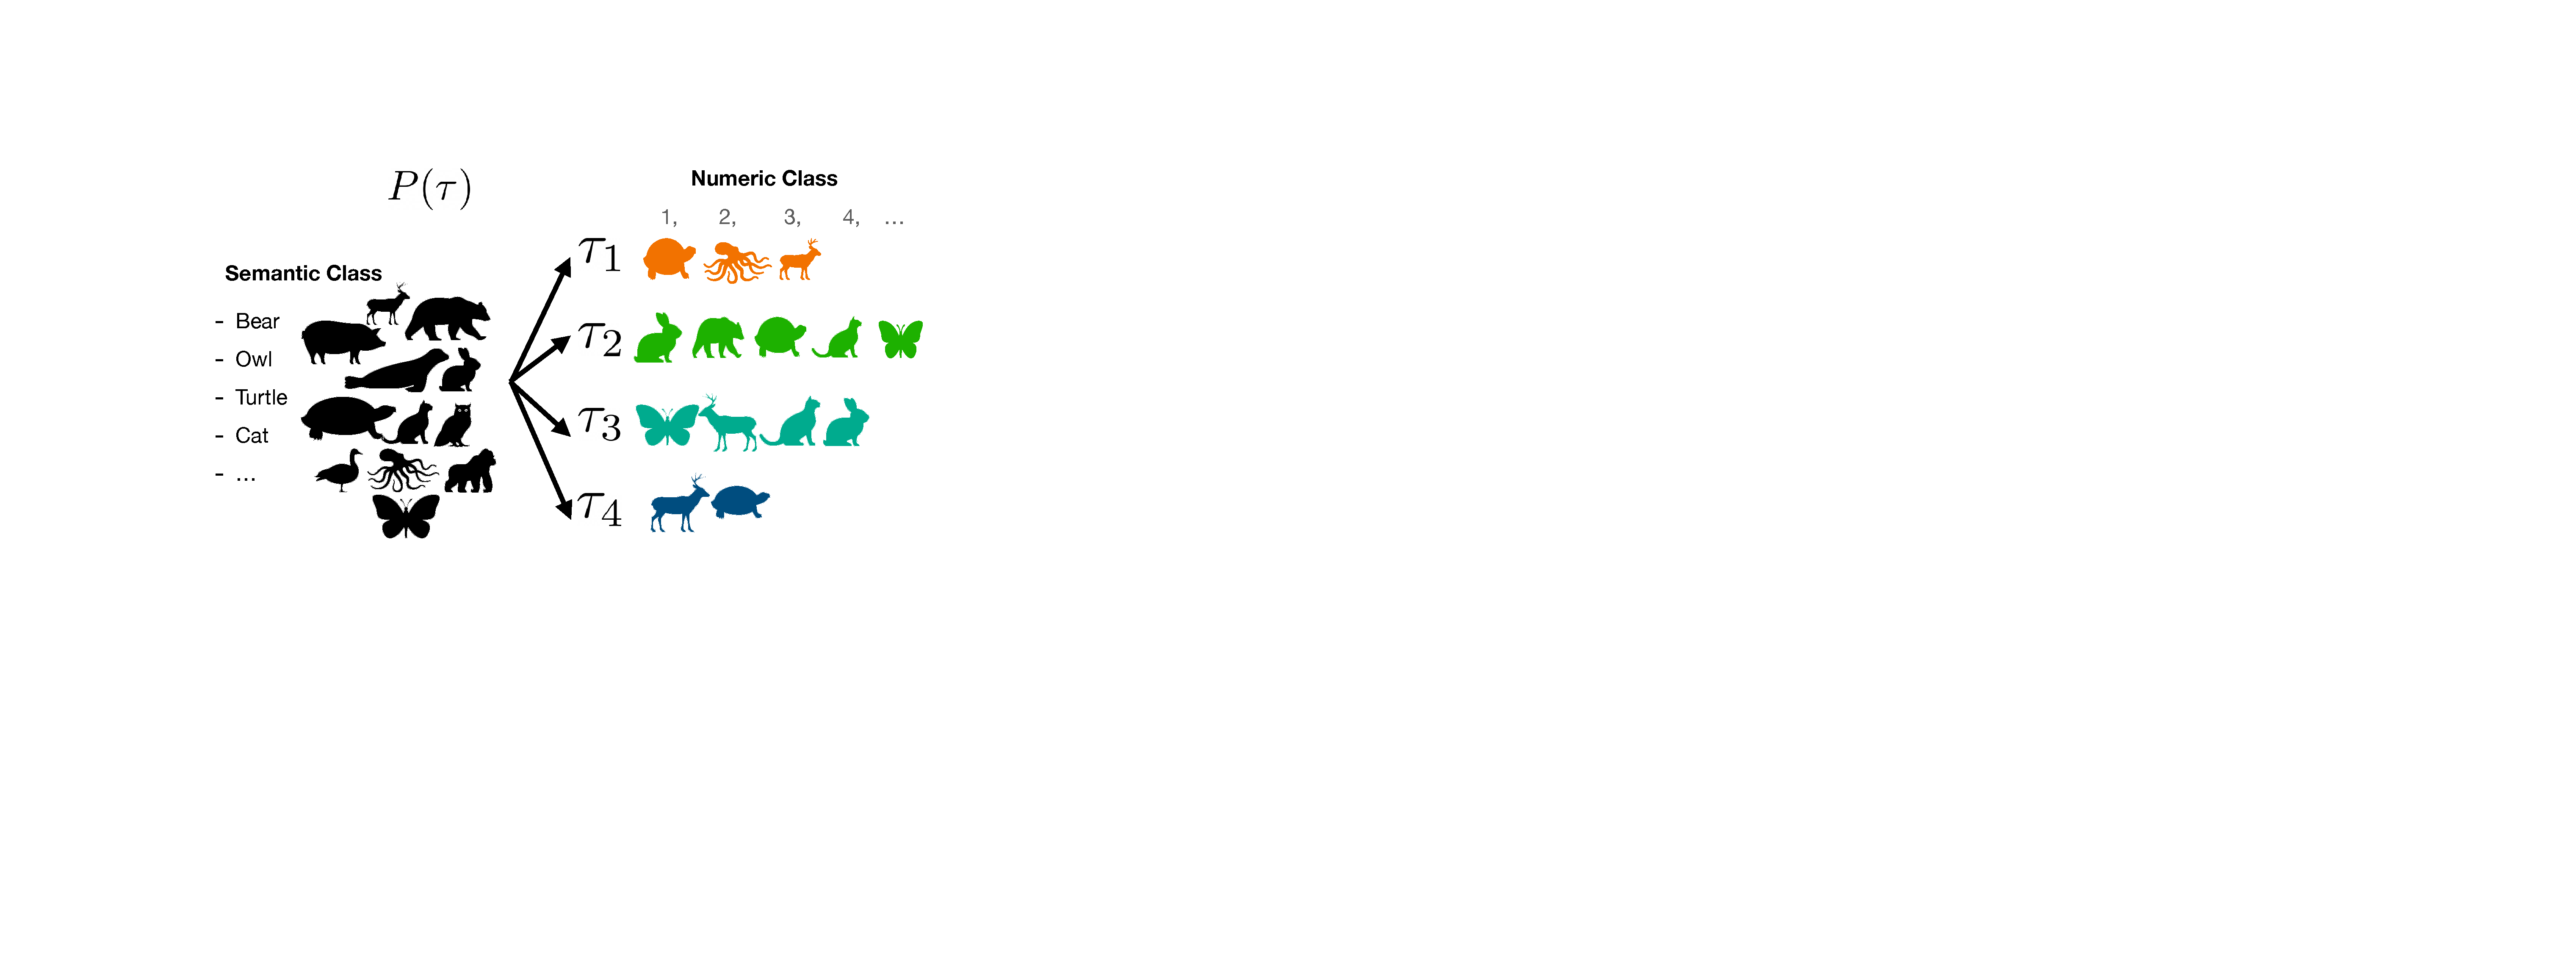
\includegraphics[width=0.4\textwidth]{figure/greenisthe.pdf}
\caption{Task sampling procedure in our \textit{any-way} meta-learning. Meta-learning employs episodic learning using a mother dataset with numerous classes ($M$) where each label represents each \textit{semantic class} (e.g. `turtle', `octopus', and `deer'). Each episode samples $N < M$ classes from this dataset and assigns a random \textit{numeric class} ($\in [N]$) to each selected class. The flexibility of our \textit{any-way} setting allows varying $N$ across tasks, distinguishing it from the conventional fixed sampling procedure.}
\label{fig:task_sampling}
\end{figure} 

There are two main meta-learning approaches. The first approach focuses on creating an effective feature extractor, like ProtoNet \cite{episodic:MBML:Protonet}, which can accurately cluster unseen instances from the same class to enable the model to generalize well to new data. The second approach aims to find a suitable initialization point for the model, facilitating rapid adaptation to unseen tasks \cite{episodic:GBML:MAML, episodic:GBML:LEO}. 

To imbue the model with meta-learning ability, both methods involve episodes. Each episode consists of multiple tasks and tests the model's meta-learning ability in the regime of few-shot learning
(Fig.\ref{fig:task_sampling}). This continuous exposure to new tasks helps the model improve its learning ability from limited data, simulating the conditions where humans learn.

Nonetheless, in contrast to the human's remarkable flexibility in classifying varying numbers of classes, the current learning models remain rigid, restricted to the fixed `way' they were trained on. As evident in Table~\ref{table:intuition}, when a model trained on 10-way-5-shot tasks from MiniImageNet \cite{dataset:MiniImageNet} is tested on a 3-way-5-shot cars \cite{dataset:cars} setting, its performance plunges to a mere 41$\%$. Considering that random sampling would yield at least 33$\%$, this reveals a glaring deficiency in meta-learning's adaptability across different `way' settings.

The sharp decline in performance is more than just a testament to the model's inflexibility; it also suggests that different `way' episodes might hail from different distributions. This variation between distributions touches upon a deeper, underlying problem: domain generalization. Essentially, to achieve true `any-way' learning, our models must address the broader challenge of performing effectively even in disparate, unseen domains.

The core objective of this paper is to highlight and address this challenge, advocating for an approach where task cardinality agnosticity becomes a foundational element in meta-learning.
To deal with this problem, we propose an \textit{‘any-way’} meta-learning method based on the concept of ‘label equivalence’, which emerges from the task sampling process, an essential element in few-shot learning including meta-learning.
The task sampling process has a unique characteristic: classes are randomly sampled and assigned to (typically numeric) class labels within each episode. These labels are not assigned based on the inherent semantics of the classes; rather, they are determined by the requirements of the specific tasks in each episode. As a result, the same class can be assigned different labels in different tasks and episodes, and the meaning of a label can change from one task to another. As a result, a numeric class label in a given task does not necessarily represent a specific class\footnote{In this paper, we differentiate the `semantic class' from the `numeric class label' as shown in Figure~\ref{fig:task_sampling}.}. This distinction introduces a phenomenon we term `label equivalence', which suggests that all output labels are functionally equivalent to one another. Although there exists a paper \cite{lee2023shot} which argues that each inner loop is equivalent to a whole training trajectory in conventional deep learning, no previous paper has developed this phenomenon in terms of label equivalence.

\begin{table}[t]
% \vspace{-3mm}
%across different number of ways, a model is trained within MiniImageNet. number in paraenthethis indicates number of shots.}
\centering
\begin{tabular}{c|cc|cc}
\hline
\# of ways (train)    & \multicolumn{1}{c|}{3} & 10    & \multicolumn{1}{c|}{5} & 10    \\ \hline
\# of ways (test)     & \multicolumn{2}{c|}{3} & \multicolumn{2}{c}{5} \\ \hline \hline
MiniImageNet (5) & 76.27      & 62.45     & 64.92     & 55.2      \\ \hline
Cars (5)        & 59.95      & 41.47     & 47.73     & 32.38    \\ \hline
\end{tabular}
\caption{Performance Comparison in MiniImageNet across different numbers of ways. The numbers in parentheses indicate the number of shots.}
\label{table:intuition}
\end{table}

Examining label equivalence naturally brings up an important question: Given the equivalence of all labels or output nodes,
%If all labels or output nodes are equivalent, 
is it necessary 
to match the number of output nodes to the number of classes in each task? For instance, if a new task consists of three classes, we can select 3 nodes from a pool of, let's say,  
% among, for example, 
30 output nodes and designate them as numeric labels, optimizing solely for this selected path. This implies that there's no need to rigidly stick to a fixed number of numeric labels, potentially allowing us to further generalize the few-shot learning process. It is from this juncture that our discourse begins.

The primary contribution of this paper is the world-premiere proposition of 
%\jh{generalized} 
`any-way' few-shot learning, moving beyond the conventional fixed-way few-shot learning. Not only do we extend meta-learning to any-way, but we also provide an efficient, general learning algorithm that achieves performance comparable to or even better % or potentially even better
than fixed-way learning. Moreover, label equivalence further suggests that individual outputs cannot represent the semantic of a class. This arises from the fact that each few-shot task %, whether episode-dependent or not, 
contains no semantic information about its class, nor does it recognize or account for the classes it comprises. From this perspective, we can perceive supervised learning as solving a given task within an absolute coordinate system (one axis for one semantic class), while few-shot learning can be viewed as problem-solving within a relative coordinate system, where the uniqueness of each class is the only clue for learning. %the only known variable is the uniqueness of each \nj{class}.} 

Our second contribution deals with the challenges arising from the lack of semantic class information. In this paper, we introduce an algorithm that compensates for this issue by integrating semantic class information into the learning process. We show that our algorithm not only improves performance in environments where the distribution of the test set differs from that of the training set, but also enables the application of data-augmentation techniques used in supervised learning to few-shot learning tasks. We demonstrate the effectiveness of this approach in MAML and ProtoNet, two of the most representative methods of episode-based meta-learning.

% Lastly, we show that these techniques are also applicable to conventional episode-independent few-shot methods \cite{}. Although episode-independent methods can sometimes outperform episode-based learning, their inherent approach of addressing the problem through the data scarcity problem makes it difficult to regard them as true meta-learning techniques. \jh{This paper, \yr{however,} shows that we can even increase the performance of episode-independent learning by injecting meta-episode semantic information only from few episodes. In essence, %we can have our cake and eat it too: 
% we can harness the benefits of the meta-learning methodology for episode-independent methods, albeit with the trade-off of using a few known episodes.}
% %\nj{*** 마지막 문장의 의미가 이해가 안 됨.***}

% \jh{The thing is both shares same episode sampling procedure. As seen in Fig.~\ref{fig:tasksampling} They do not have any information of given episode(Task? Episode? 통일 필요). Also, each class can be assigned to different label in different episode. In this paper, we focus on this phenomenon. We will call this phenomenon as 'label equivalence'. Which means no label is more different than others. Every label is equivalent to others. As this phenomenon is more important to episode-dependent meta learning. We will focus more on this. However, we also deal with episode-independent meta learning by using episode-dependent feature to it.}

% \jh{Also, this task set sampling methodology lacks class information. Even if the task-label set is fixed, each label is only a match to the task-label in that task (episode), and the neuron does not store any special information. Let's compare this phenomenon to supervised learning.  This does not happen in supervised learning. If we assign class A to output 0, then output 0 represents class A. What this means is that the initial state of the output neurons before learning a new task is not different from each other. We will refer to this phenomenon as label equivalence.}
% \jh{In this paper, we focus on label-equivalence because it is a unique phenomenon in few-shot learning. In this paper, we analyze this phenomenon and propose a way to take advantage of it. As a result, our paper aims to provide one insight into few-shot learning based on the keyword label equivalence.}
% \jh{이를 살펴볼 때, 먼저 이전에 episode-learning based 모델의 경우 진짜 meta-learning ability를 가지고 있는 것에 가깝다고 했지만, task-label의 개수가 fixed되어 있다는 조건 때문에 진정한 meta-learning 능력을 가지고 있다고는 의문이 있음. 이는 애초에 desired way의 크기를 키운 다음에 더 작은 incoming task set에 대해서 inference하면 된느거 아닌가? 하는 의문이 생길 수 있지만, 이는 후술하겠지만 일반적으로 episoded-based 모델의 경우 학습한 way set 에 대해서만 성능이 나오고, 이와 다를 때 성능이 급격히 떨어지는 경향을 보임. }
% \jh{Task set을 sampling 하는 점의 특징은 이 뿐만이 아님, 왜냐하면 이렇게 task-label set을 고정해놓는다고 하더라도 , 각각의 label은 해당 task(episode)에서의 task-label을 맞추는 것일 뿐, 해당 neuron이 특별한 정보를 저장하는 것이 아니기 때문. 이 현상이 무엇인지 supervised learning과 비교해 보겠음.  supervised learning에서는 이러한 현상이 일어나지 않음. 만약 0번째 output에 class A를 assign해주었다면 0번째 output은 class A를 represent함. 이는 무엇을 의미하냐면, 새로운 task에 대해서 학습하기 이전의 초기 상태는 output neuron 서로 다르지 않다는 것임. 본 논문에서는 이러한 현상으f label equivalence로 지칭하겠음.}
% \jh{본 논문에서는 label-equivalence에 집중할 것인데, 왜냐하면 이러한 현상은 supervised learning의 일종이라고 볼 수 있는 few-shot learning의 고유한 현상임에도 불구하고, 이 equivalence 자체에 대해서 집중한 페이퍼는 거의 없었기 때문임. 본 논문에서는 이러한 현상을 분석하고, 또 이 현상에서 advantage를 얻을 수 있는 방법을 제시하고자 함. 결과적으로 우리의 논문은 few-shot learning에 대해서 label equivalence라는 키워드를 바탕으로 하나으ㅣ insight를 제공하고자 ㅎㅏa.}
% \jh{label equivalence를 살펴보았을 때, 다음과 같은 질문은 자연스러움. 어차피 각 neuron이 equivalent하다면, 굳이 매 task에서 neuron의 개수와 task label의 개수를 맞출 필요가 없지 않은가? 만약 새로운 task의 label set이 3개라면, 우리는 output neuron중에서 3개를 골라서 이를 task-label이라고 하고 이 selection path에 대해서만 optimization을 하면 됨. 그렇다면 우리는 굳이 fixed-number of task label에 집착할 필요가 없으며, 더 나아가 few-shot learning의 과정을 좀더 일반화할 수 있음. 우리의 이야기는 이곳에서 시작됨. 우리의 첫 번째 contribution은 기존의 fixed-way few shot learning이 아닌, any-way few shot learning을 제시한다는 것. 우리는 단순히 any-way로 늘리는 것 뿐 아니라, 매 way의 성능이 fixed-way의 성능과 유사한 수준으로 만들어주는 이에 맞는 적절하고, 일반화된 학습 알고리즘을 제시하며, 오히려 fixed-way보다 성능이 더 좋을 수도 있다는 것을 보여줌 (이부분은 아직 데이터가 다 안나와서.. 추후 맞춰서 수저ㅇ)}
% \jh{label equivalence는 또한 각각의 ㅐutput들이 class를 represent 할 수 없게 만듬. 이는 왜냐하면 episode-dependent하든, 아니든 간에 매 task 에 대한 정보는 전혀 없고, 또한 그 task가 실제로 어떤 class를 가지고 있는지는 전혀 상관이 없고, 또 모르기 때문. 이러한 현상을 놓고 본다면 supervised learning에 비해서 few-show classification task는 제공받는 정보의 차원이 하나 더 낮다고 생각할 수 있음. 비유하자면 supervised learning은 절대 좌표계 속에서 주어진 task를 푸는 거라면 few-shot learning의 경우는 각 task들이 서로 다르다는 사실만 알 고 있는, 상대 좌표계 속에서 문제를 푸는 것으로 보임. 본 논문에서는 해당하는 문제를 보완하여 학습 과정 속 ㅊlass-label information을 inject하는 알고리즘을 제시하였으며, 이 알고리즘이 training set과 distribution이 비슷한 test set이 아닌, distribution이 다른 더 practical한 환경에서도 마찬가지로 성능 개선을 늘릴 수 있음을 보여줌. 또한, 이를 통해서 few-shot learning task에 supervised learning에서 사용하는 기법ㅇ들을 적용할 수 있음을 보여줌. 위의 두 방법들에 대해서는 episode-based learning에서 가장 대표격인 MAML, ProtoNET에서 이것이 작동함을 보였음.}
% \jh{본 논문에서는 마지막으로 이러한 기법들이 episode-independent한 기법에 대해서도 적용 가능하다는 것을 보여줌. 기존의 episode-independent한 기법은 성능 면에서는 episode-based learning보다 도 좋을 수 있지만, 결국 이를 ㅇataset scarcity problem을 통해 문제를 풀기 때문에 이를 true meta learning 기법이라고 보기에는 무리가 있음. 본 논문에서는 특정한 제약조건을 추가하였을 때 모델이 previous episode에서 학습하여 크게 성능을 개선할 수 있음을 보여줌.}
% \jh{정리하자면, 본 논문에서는 task sampling method에 주목하였고, 이를 통하여 meta learning 기법들을 더욱 더 일반화하였으며 기존의 방식보다 더 인간의 classification 방식에 더 가까운 방식을 제안하였음. 우리는 앞으로도 ㄹew-shot classifciation에서 우리의 방법이 baseline으로 사용되어 더 일반화된 메타 능력 측정 방식이 되기를 기대함.}

% 맨 마지막 두 문단은 어감이 이상해서 추후 수정하게Ttmqslek.
% 이 다음, GBML에 대한 조금 더 자세한 설명, 이후 특별한 feature가 task sampling procedure라는 것을 언급.
%\jh{GBML aims to train a meta-learner, \ie an initialization point which can adapt unseen classes using a few examples within a few gradient steps. \nj{For this}, GBML adopts a special procedure \nj{that}}
%\jh{\nj{samples a random} task from a task distribution and the classes in the sampled task
%are randomly assigned to labels (e.g., an integer). %This \nj{endows} a label \nj{an interesting characteristic}. Each label does not represent a specific class. This leads to a equivalence \nj{?? . That is, no label is more important, or different
%than others. 
%num-way에 대한 설명, 근데 이게 좀 사람들이 듣기 어렵지 않나. 해당 way보다 더 많은 way로 학습할 수 있는

% \jh{First feature of this equivalence implies that we do not need same number of neurons to the number of labels of episode. This is because as every label is no more different than other}
% \jh{따라서 우리는 다음과 같은 구조를 생각할 수 있다. 각 episode를 풀 때에, 여러개의 output index 중에서 해당 task를 풀 output index를 랜덤하게 정하게 되면 어차피 label간의 equivalence가 보장되기 때문에, output dimension이 task label set보다 더 커도 상관이 없다는 것이다. 따라서 우리는 해당 사실을 바탕으로 기존의 episode-dependent meta learning task를 조금 더 일반화 할 수 있다. Fig.\ref{fig:our_architecture}처럼. 즉 classifier가 존재하는 경우, classifier set의 task label set으로 전사하는 과정을 넣음으로서 meta-learning architecture에 조금 더 유연성을 추가할 수 있다.}
% \jh{task-label set보다 많은 classifier neuron의 존재는 단순히 모델의 유연성 뿐 아니라, (해당 way보다 더 많은 way로 학습할 수 있다 라는 말을 하고싶음). 기존 task보다 더 큰 set, 다시 말해, classify해야 하는 class의 수가 더 많은 set도 풀 수 있다는 것을 의미한다. 기존의 episode-dependent는 stream of episodes로 학습하기 때문에, 각 task의 label set의 크기가 같았고, 따라서 해당 model은 episode와 같은 shape를 가진 task만 풀 수 있었다. 하지만 이러한 label equivalence에 대한 분석을 바탕으로 우리는 최초로 fixed-way (\ie task label의 크기가 같은) 문제만 풀 수 있는 episode-dependent 모델이 아닌 any-way 문제를 풀 수 있는 episode-dependent 모델을 제안한다.}
% % Because the real class has no fixed relation to the assigned label in a task, every label is equivalent to others in that the assignment of a class to different labels should not make any difference. 
% This feature is unique to GBML. Although GBML relies on the same framework as supervised learning, only GBML has this feature which makes it special. In this paper, we focus on this equivalence among labels and seek how to use this specific feature and argue that this feature can be used as a double-edged sword boosting the performance of GBML if properly utilized.}
\begin{figure*}[!ht]
\centering
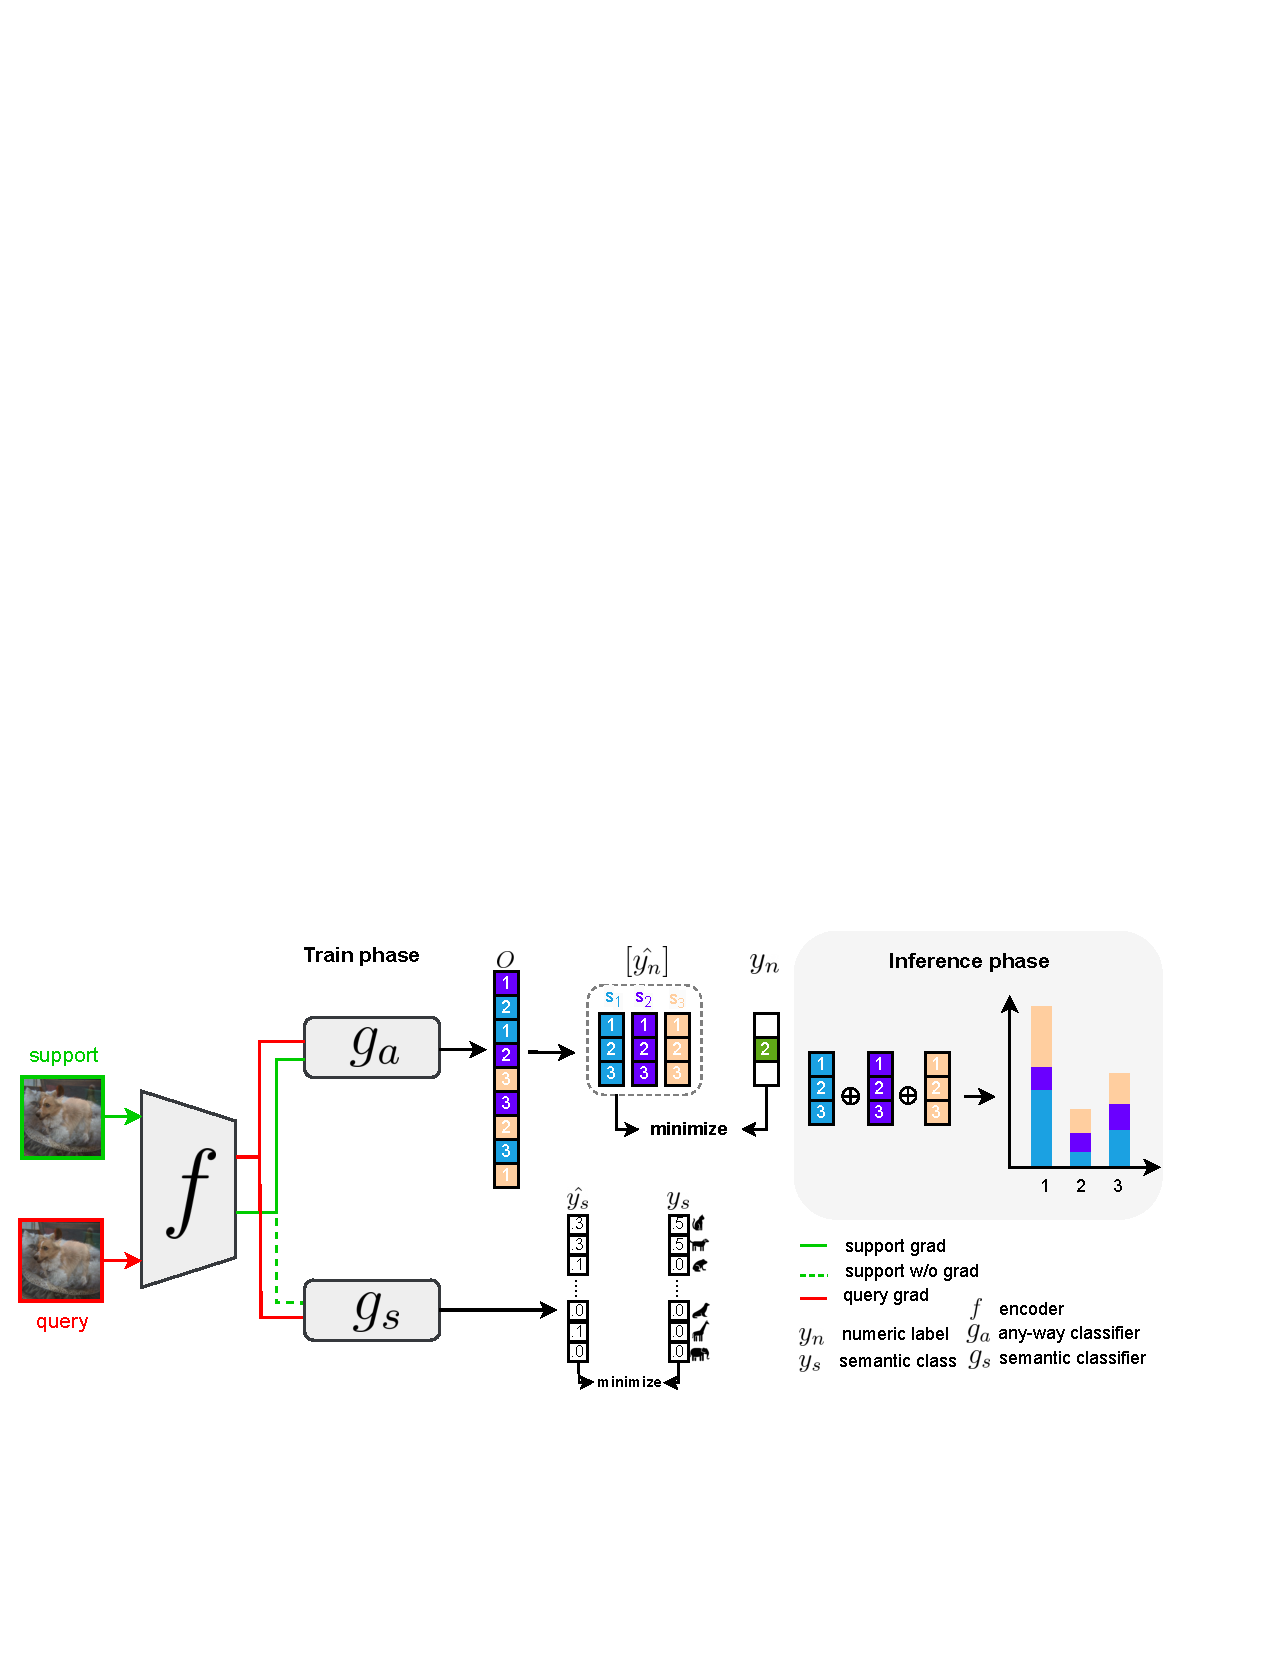
\includegraphics[width=\textwidth]{figure/realfinallyfinishedfinalalgir.pdf}
\caption{Overall structure of our proposed algorithm. The upper section outlines the implementation of the any-way meta-learning, while the lower section highlights the integration of semantic class information. Note that the encoder $f$ is not updated with the semantic classifier $g_s$ during the inner loop (dotted green line). For mixup input, a separate numeric label is assigned in $g_a$, while traditional mixup training is done in $g_s$.}

\label{fig:our_architecture}
\end{figure*}

% \jh{The equivalence \nj{among labels} itself can give some flexibility to the model. For example, it could fit any type of class. That is, once it is trained well, it could fit any dataset. \nj{*** fit dataset ***의 의미가 모호함.} \cite{asd} shows that it not only fits the dataset but also leads to good performance. In this paper, we focus on this flexibility, we aim to give more flexibility to GBML by \nj{exploiting} this equivalence. \nj{First, we} propose a \nj{GBML method that} can classify any number of classes. That is, suppose the model is trained to classify 5 classes, traditional GBML, or any supervised learning and its variants, can only classify 5 classes. However, our method can classify any number of classes more than 5 without sacrificing performance. Also, we would introduce some masking techniques that can improve the performance and dynamics of the model based on our algorithm.}

% 둘째로, 이러한 label equivalence한 성질은 문자 그대로 label이 한 class를 대표하지 않는다는 것을 알 수 있는데, 이는 'learning from data'라는 가장 기본적인 컨셉에서, data의 정보량이 episode-dependent한 학습 방법론은 class-label matching이 가능한 supervised learning보다 떨어진다는 것을 의미한다. 개는 첫번째 인덱스에 올 수 도 있고, 두번째 인덱스에 올 수 도 있기 때문이다.

% 본 페이퍼에서는, 메타 러닝에서 이러한 현상이 성능에 장애가 될 수 있음을 처음으로 제안하고, Episode-dependent한 학습 방법론에 label information을 추가적으로 넣음으로서 이를 해결하고 성능을 전반적으로 올릴 수 있는 단순하지만, 추가적인 연산량이 많이 필요하지 않은 방법론을 처음으로 제안한다. 또한 이러한 supervised learning 성질을 추가함으로서, 우리는 episode-dependent meta learning에 supervised learning에서 자주 사용하는 trick을 쓸 수 있음을 보인다. 이는 supervised learning에서 자주 사용하는 기법 중 하나인 mixup을 사용하여 성능을 전반적으로 올림으로서 증명한다. 또한, label information을 사용한다고 하더라도 성능 개선이 dataset-specific하게 이루어지는 것이 아님을 본 페이퍼에서 증명한다.

% 반면, episode independent한 method의 경우 위에서 언급했던 문제와는 관련이 없다고 이야기 할 수 있는데, 왜냐하면 해당 현상은 전부 episode를 통해서 학습함으로서 벌어지기 때문이다. 따라서 episode를 통해서 sampling하지 않는 방법들 \cite{rethinking..}은 이와 관련이 없다. 하지만, 반면에 이러한 방법론들은 문제를 해결하는 것을 단순히 양적으로 encoder를 좋게 만든다던가, few-shot example의 양을 늘림으로서 해결하는 등의 meta-learning이라는 essense와는 떨어지는 것이 사실이다. 따라서, 본 논문에서는 아주 작은 수준의 추가적인 조건만 가지고 episodic 한 성질을 inject하고, 성능을 드라마틱하게 개선할 수 있는 방법을 제안한다.
% % \jh{\nj{secondly,} we will address that this equivalence naturally leads to a lack of information. That is, as all labels are equivalent, the assigned 
% target label lacks information about the exact class of the sample in question. For example, in any traditional supervised learning, each class represents
% a specific class and a model can learn about the class by classifying each input to the corresponding class. However, in GBML, as \nj{all the labels are} equivalent, the model cannot learn about the specific class to which a sample belongs. %In other words, the model lacks information on that class compared to supervised learning. 
% In this paper, we are to solve this problem by injecting label information into the model. Our algorithm does not require specific architecture or a huge computational \nj{overhead}. Also, injecting label information means that we can make use of the techniques utilized in supervised learning such as \cite{mixup, } in GBML. In this paper, we propose to apply Mixup \cite{mixup} technique to GBML and show that it improves the performance. It suggests that some techniques of supervised learning can be applied to GBML within our framework.}
% % 본 페이퍼에서, 우리는 가장 대표적인 episode-dependent paper인 MAML에 우리의 방법론을 적용해보고, 우리의 방법론이 잘 work한다는 것을 보일 것이다. 그리고 우리의 방법론이 몇가지의 가벼운 조건만 있으면 우리의 방법론이 episode-independent에도 적용 가능하다는 것을 선보일 것이다.

% 우리 페이퍼가 전반적으로 넓은 분야를 지칭하기 때문에, 해당 분야에 대한 설명을 Related Work에서 하도록 한다.
\section{Related Works}
% 메타 러닝에 대한 간략한 설명, 무엇을 이야기해야 하냐면, 이것의 목표는 뭐고, 대부분은 무엇무엇을 다룬다. 어떤 모델이 메타 러닝 능력을 가지고 있다고 이야기하기 위해서라면, 일반적으로 그 모델은 몇 개의 샘플들만 가지고 그 샘플들간의 관계에 대해서 알 수 있어야 할 것이다. 이런 개념을 \cite{labelequiv:metadefinition}에서 정의하였으며, 다음과 같이 meta-learning ability를 지속적으로 체크하며 직접적으로 성능을 발전시키는 매커니즘을 \cite{label_equiv:matchingnetwork}에서 제안하였다. ㅐ해당 논ㄴ문에서는 각각 작업을 풀기 위해서 작은 데이터셋 (support set)을 사용하는 episodic training 방식을 도입하였다. 

% \subsection{Episode-based Meta Learning}
% Matching network \cite{label_equiv:matchingnetwork}을 필두로 하여, 현재의 대부분의 메타 러닝 모델은 episode-based로 학습한다. \cite{nonepisodic:transferminitocars}가 정리한 것처럼, 대부분의 episode-based model의 경우 meta learning 능력을 얻기 위한 meta-training stage, 그리고 이 성능을 테스트하기 위한 meta-test stage로 이루어져 있으며, 크게 두 가지의 방식의 접근법이 사용된다

% 첫째 방법론은 Gradient-Based Meta Learning이다(GBML) Model-Agnostic Meta-learning model(MAML) \cite{episodic:GBML:MAML}이 첫 번째로 제안하였으며 해당 방식은 support set을 inner loop에서 gradient descent로 학습하고, 얼마나 잘 optimized 되어 있는지를 query set에서 학습한 후, 더 support set을 잘 학습하도록 outer loop에서 meta-initialization paremeter를 학습시킨다. GBML이라고 불리는 연구는 많이 이루어지고 있으며 \cite{episodic:GBML:ANIL, episodic:GBML:imaml, episodic:GBML:warpgrad, episodic:GBML:Reptile} 이때 inner loop에서의 성능을 계산할 때 Hessian을 계산해야 하기 때문에 이것의 계산량을 latent vector를 이용하여 줄이거나 \cite{episodic:GBML:LEO}, 혹은 Hessian을 이용하지 않는 방법들이 연구되어왔다 \cite{episodic:GBML:ANIL, episodic:GBML:Reptile, episodic:GBML:MAML}. 
% 두번째 방법론은 Metric-Based MEta Learning (MBML)으로서, 좋은 encoder를 학습하여 feature 단에서 잘 clustering 되도록 하는 것이 목표이다.  \cite{label_equiv:matchingnetwork} 등에서 시작하였으며, GBML 이전부터 사용되던 방법론이다. Protonet \cite{episodic:MBML:Protonet}이 기초가 되는 아키텍쳐를 제안하였으며, 이는 support set에서 encoder를 뽑은 다음에 clustering한 다음, query set에서 해당하는 class와의 거리를 줄이는 것을 방법론으로 한다. 이때의 clustering은 Euclidean space에서 했는데, 이것은 Hyperbolic space와 같은 다른 Riemannian 공간에서 해도 잘 된다. \cite{episodic:MBML:Hyperbolic}
% \subsection{Transfer-Learning Based few shot learning}
% MBML은 때로는 단순히 좋은 encoder를 unsupervised 단에서 잘 만들도록 하는 문제에서 지표를 측정하는 metric으로 분류되기도 한다. \cite{nonepisodic:transferisbetter}가 제안하였듯이, 이 문제를 meta-learnin 문제가 아닌 few-shot learning으로 보게 된다면 encoder를 잘 학습하고, 그리고 transfer learning에서 dataset scarcity problem으로서 볼 수 있게 된다. 이러한 방법들의 공통점은 결국 unsupervised manner에서 문제를 풀어야 한다는 것인데, 이 문제를 해결하기 위하여 이들은 label에 의존하지 않고 새로운 문제를 만들어 그 문제를 풀도록 한다. 이들은 보통 두 개의 같지만 다르게 표현된 이미지를 encoder가 같게 만듦으로서 문제를 푼다 \cite{label_equiv:ssl:byol,label_equiv:ssl:simclr}. 예를 들어서 self-supervised learning의 경우 이미지를 마구 뒤섞어 직소 퍼즐을 맞추는 식으로 바꾸거나 \cite{label_eqiv:ssl:jigsaw}, 혹은 사진을 뒤집고, 회전하여도 같은 이미지라고 보게 하거나, \cite{label_eqiv:ssl:rot} 결국에 \cite{label_eqiv:ssl:rot,label_equiv:ssl:byol}. 이렇게 학습시킨 후, 실제 데이터셋으로 들어가기 전 모델은 classifier를 학습하는 transfer learning을 거친다. 

% 여기서 주목할만한 점은, 이 문제를 transfer learning으로 바꾸어서 풀게 되더라도 결국에는 label information이 없기 때문에 어떤 task를 풀기 위해서 절대적인 class를 represent하는 semantic class supervised learning을 거친다는 점이다. 이는 task로만 학습해서 develop하는 episodic learning과는 대비된다. episodic learning에서는 semantic class가 사용되지 않고, 각 task에서 numberic label만 랜덤하게 배정된다.
% \subsection{Meta Learning} \yr: 이렇게 하는 건 별로야? ㅎㅁㅎ
\paragraph{Meta-Learning,} briefly described, is about the study of algorithms that learn from data. As defined in \cite{labelequiv:metadefinition}, the fundamental concept of meta-learning is the model's capability to discern relationships among a limited number of samples.
%The crux of meta-learning is the capability of a model to discern relationships between a limited number of samples. This fundamental concept of meta-learning was defined in \cite{labelequiv:metadefinition}. 
Furthermore, mechanisms were proposed in \cite{label_equiv:matchingnetwork} to continuously verify meta-learning abilities while simultaneously enhancing performance.
%mechanisms that continuously verify meta-learning abilities while directly enhancing performance were proposed in \cite{label_equiv:matchingnetwork}. The latter introduced the episodic training method, employing a small dataset, termed the support set, to tackle each task.

Inspired by the Matching network \cite{label_equiv:matchingnetwork}, a majority of current meta-learning models have adopted an episode-based training approach. As summarized by \citet{nonepisodic:transferminitocars}, these episode-based models usually consist of two stages: the meta-training stage to acquire meta-learning capabilities, and the meta-test stage to evaluate their performance. There are two lines of research in this area:

% \paragraph{Gradient-Based Meta Learning (GBML)} %This methodology,
\paragraph{Gradient-Based Meta Learning (GBML)} %This methodology,
 introduced by the Model-Agnostic Meta-learning model (MAML) \cite{episodic:GBML:MAML}, it involves training the support set in the inner loop through gradient descent. The degree of optimization is then evaluated on the query set, followed by the outer loop refining the meta-initialization parameter to enhance learning on the support set. %The degree of optimization is then gauged on the query set, after which the outer loop refines the meta-initialization parameter to improve learning on the support set. 
There's a growing body of research in GBML
%, as evidenced by works 
such as \cite{episodic:GBML:ANIL, episodic:GBML:imaml, episodic:GBML:warpgrad, episodic:GBML:Reptile}. Notably, due to the computational demands of caluculating the Hessian in the inner loop, %performance computation, 
methods that utilize latent vectors to reduce this computation %to reduce this computation using latent vectors 
have been explored \cite{episodic:GBML:LEO}. Other studies have put forward the idea of % Other research efforts have proposed 
avoiding the use of the Hessian altogether \cite{episodic:GBML:ANIL, episodic:GBML:Reptile, episodic:GBML:MAML}.

\paragraph{Metric-Based Meta Learning (MBML)} is focused on training an effective encoder that can perform clustering at the feature level. This approach, which predates GBML, was established by initiatives such as \cite{label_equiv:matchingnetwork}. 
%Initiatives such as \cite{label_equiv:matchingnetwork} set the foundation for this methodology, which predates GBML. 
A foundational architecture for this was proposed by Protonet \cite{episodic:MBML:Protonet}. The method involves extracting features for the inputs in the support set by an encoder, clustering them, and then minimizing the distance between the query set and the corresponding class. Although clustering is conventionally conducted in the Euclidean space, it has been shown to be more effective in other Riemannian spaces like the Hyperbolic space \cite{episodic:MBML:Hyperbolic}.

\paragraph{Domain Generalization} 
This field focuses on designing models that exhibit robustness across diverse environments~\cite{DG:Gunbon0,DG:Gunbon1}. Our approach to ``any-way" meta-learning aligns with this objective. As illustrated in Table~\ref{table:intuition}, episodes of varying cardinality can be perceived as from distinct distributions. In pursuing a model endowed with a genuine meta-learning capability— capable of adapting to any task cardinality— we inevitably confront the challenges posed by domain generalization.

The conventional understanding suggests that while it is possible to enhance the overall performance on a set of tasks, the performance on individual datasets might decline %may suffer
when compared to models trained exclusively %solely 
on a specific episode~\cite{DG:wisdom0,DG:wisdom1,DG:wisdom2}. In this paper, we challenge this established notion. %conventional wisdom.
Through the integration of label equivalence, we posit that this trade-off might not be as significant %pronounced 
within the meta-learning realm. Our results exhibit not only the seamless adaptability to ``any-way" tasks but also superior performance compared to fixed-way training paradigms.

% \jh{\textbf{Transfer-Learning Based Few-shot Learning}
% Sometimes, MBML is categorized as a metric to \yr{evaluate} the quality of an encoder crafted in an unsupervised manner. As suggested by \cite{nonepisodic:transferisbetter}, if this challenge is viewed not as a meta-learning problem but as a few-shot learning task, the focus shifts to proficient encoder training. Furthermore, it sees the challenge from a transfer learning perspective, addressing the dataset scarcity problem. A common theme across these methods is solving the problem in an unsupervised fashion. They construct novel problems that don't rely on labels. For instance, in self-supervised learning, strategies like rearranging images to match jigsaw puzzles \cite{label_eqiv:ssl:jigsaw}, or ensuring encoders perceive flipped or rotated images as identical \cite{label_eqiv:ssl:rot, label_equiv:ssl:byol}, are commonly employed. After such training, the model undergoes transfer learning by training a classifier before interacting with the actual dataset.
% }
% \jh{An essential observation here is that even when reframing the problem through transfer learning, there's an inherent dependency on semantic class supervised learning due to the absence of label information. 하지만, few-shot classification을 할 때에 있어서는 그러한 과정이 생략된다. This is in contrast to episodic learning where semantic classes aren't used, and numeric labels are randomly assigned for each task.}
% \jh{또 하나의 중요한 점은 few-shot classification 능력을 측정할 때에는 동일한 sampling mechanism을 가진다는 점이다.}
% \section{Preliminaries}
% \begin{itemize}
%     \item Gradient-based Meta Learning
%     \item inner loop 설명
%     \item fixed-way 설명
%     \item equivalence 다시 설명 
%     \item true label, meta label 정의 필요, task-label, class-labelk
% \end{itemize}
\section{Method}
\subsection{Conventional (Fixed-Way) Meta-Learning}
% \begin{figure*}[h!]
% \centering
% \includegraphics[width=\textwidth]{figure/sampling_algorithm.png}
% \caption{\jh{sampling algorithm. By doing so, every classifier can backpropacate in every episode(task)}}
% \label{fig:masking? procedure}
% \end{figure*}

To evaluate the few-shot learning ability within a given distribution, we define a process of task sampling. Initially, 
%Firstly, 
we select a label set from the class pool of a larger mother dataset  $\mathcal{D}$. In conventional meta-learning, the cardinality $N$ of the selected label set remains
%is
fixed during the entire training procedure. We then sample data from this set, each matching the size of the support set (number of shots).
Each task $\tau$ consists of a set $\mathcal{X}$ of tuples $\{(x, y)\}$ sampled from $\mathcal{D}$, where $x$ denotes the input data and $y$ represents the numeric label rather than the semantic class from the dataset (Fig. \ref{fig:task_sampling}).  Moreover, $\mathcal{X}$ is divided into a support set $\mathcal{X}_s$ and a query set $\mathcal{X}_q$ for task learning and performance evaluation, respectively. % 이렇게 쓰는 건 어떨까?
% 기존: Moreover, $\mathcal{X}$ is partitioned into a support set $\mathcal{X}_s$ used for learning the task and a query set $\mathcal{X}_q$ \yr{for performance evaluation.} <- to evaluate its performance. ( for ~, 구조 맞추고 싶어서 ㅎㅁㅎ)
To do so, a model with encoder $f$ and $N$-way classifier $g_{f}$\footnote{$f$ denotes `fixed-way' while $a$ is used for `any-way'. } learns from the support set, then evaluates its performance with the query set.

% \jh{우선, 우리의 모델은 Output dimension $O$의 크기가 task label set의 크기보다 크기 때문에 매번 Task를 뽑았을 때 $O$중 Task label에 해당하는 $|T|$개의 label set을 selection하는 과정을 가져야 한다. 또한 equivalence를 유지하기 위해서 매번 새로운 Episode마다 $O$중 $|T|$를 sampling하는 sampling combination $s$는 $C(|O|,|T|)$에서 random하게 뽑는다.}
\begin{algorithm*}
\caption{Any-Way Meta-Learning}\label{alg:AnyWayMetaLearning}
\begin{algorithmic}

\Require Output dimension $O$ %, number of class in a task $N$} %classifier nodes set $C$, task set $t$
\Ensure Trained model $\theta$
\State Initialize model parameters $\theta$
\For{episode $= 1$ to $K$}
    \State Sample a random number $N \le O$
    \State Sample a task $\tau$ with $N$ number of classes and set $J = \lfloor O/N \rfloor$.
    \State Generate $S = \{s_j\}, j \in [J]$ where $s_j \in \mathbb{R}^N$ is a random assignment, non-overlapping with $s_i, \ \forall i\neq j$ 
    %\State Calculate $S(g(f(x_{\text{support}})))$, which has dimension $(\lfloor\frac{O}{|T|}\rfloor, |T|)$
    \State Calculate any-way loss in the inner loop: $L_{a\_in} = \sum_{j=1}^J L(S_j(g_a(f(x_{support})), \theta),y)$ 
    \State update  $\theta$ using $L_{a\_in}$ to $\hat{\theta}$
    \State Calculate any-way loss in the outer loop: $L_{a\_out}$ $=\sum_{j=1}^J L(S_j(g_a(f(x_{query})), \hat{\theta}),y)$
    %\State Initialize logit $\in \mathbb{R}^N$ to zero for performance testing with query set
    %\State $\text{logit} \in \mathbb{R}^N$
    %\For{each $j$ in $J$}
    %    \State $\text{logit} \mathrel{+}= S_j(g(f(x_{\text{query}})))$
    %\EndFor
    \State Update meta-parameters $\theta$ using $L_{a\_out}$.
\EndFor
\State \textbf{return} trained model with parameters $\theta$
\Ensure Test a model with trained model $\theta$
\State Sample a task $\tau$ from test pool and set $J = \lfloor O/N \rfloor$ and Generate $S$ in same manner. Then , update $\theta$ to $\hat{\theta}$ with $L_{a\_in}$
\State Calculate ensembled logit: $logit$ = $\sum_{j=1}^J S_j(g_a(f(x_{query})))$ to achieve test accuracy
\end{algorithmic}
\end{algorithm*}

\subsection{Any-Way Meta-Learning}\label{sec:anywaymetalearning}
As mentioned earlier, there exists an equivalence among numeric labels. % between은 둘 사이 느낌이고, among은 좀 더 여럿. numeric labels면 among이 맞지 않을까?
We can leverage
% exploit은 뭔가 착취?하는 느낌 
these characteristics to enhance the meta-ability of the model.

% a task-classifier $g_t$ that classifies these features into task-labels, and a sampling procedure, denoted as $s$. The function of $s$ is to identify the index in the output $O$ of $g_t$ that corresponds to the task-label. Mathematically, this is expressed as $s(g_t(f(x)))= { g(f(x))[i] : i \in s}$, where $s$ belongs to the set of combinations $C(|O|,|T|)$. Here, $C(|O|,|T|)$ refers to all possible ways of selecting $|T|$ elements from a set of $|O|$ elements. Usually, the output dimension of $g_t$ matches the task-label space set, implying that $s$ is a complete set selection. 
% \jh{In this paper, we introduce two significant modifications to the conventional approach. Firstly, we incorporate task cardinality as a variable in our task sampling process during training. Secondly, we expand our model by integrating a class-classifier, $g_c$, specifically designed for class-label classification.}

Firstly, our model's output dimension, $O$, is set to be greater than the maximum cardinality of the tasks' label sets, implying that each time we sample a task $\tau_i$ with $N_i$ classes, we must assign $N_i$ labels among $O$ output nodes. % corresponding to the task label. This assignment should be random to maintain equivalence.

%for each new episode, we randomly select labels. Which means, we draw a random sampling combination $s$ from $C(|O|,|T|)$, where $s$ indicates the $|T|$ labels from $O$.}
With our proposed configuration, we maintain output-to-class assignments during each episode. This not only determines a unique and unchanging pathway for selecting numeric labels but also restricts gradient updates to occur exclusively along this fixed way, thereby accommodating the execution of standard meta-learning tasks. Unlike traditional methods that fix the cardinality of the task when conducting task sampling, our approach also involves sampling the cardinality. % yr: 문장 호흡이 너무 길어서 나눔
This enables our model to handle tasks with any cardinality, hence fostering a cardinality-independent learning environment, \ie any-way meta-learning. 
%\yr{learning environment that is independent of cardinality, \ie any-way meta-learning.}

However, a potential problem can arise when the output dimensionality $O$ significantly exceeds the expected task cardinality. In this case, the chance of each classifier node being selected %to classify the task 
in each episode approaches zero. Consequently, classifier nodes might undergo less training than the encoder throughout the training procedure, resulting in an underfit.
%at $\frac{|O|}{\mathbf{E}(|T|)}$. Should this probability be low, classifier nodes might undergo less training than the encoder throughout the learning process. In this paper, we introduce a simple yet effective remedy to counteract this problem.
To remedy this, we assign a set of output nodes to a numeric label. We assign a numeric label to (almost) all nodes for classification, rather than assigning a numeric label to just one output node and ignoring the unassigned nodes.
% \yr{rather than? 을 말한 이유 잘 모르겠음. to clarify? 아니면 기존엔 저렇게 해?} Rather than assigning \nj{a numeric label to only one output node} %three output nodes \nj{to the three numeric labels} 
%and ignoring the \nj{unassigned \yr{nodes}}, we propose assigning a numeric label to all nodes for classification.

Let $f(x)$ be a feature map for the input $x$ and $g_a(\cdot)$ be an any-way classifier consisting of $O$ output nodes. For a task with $N$ classes, we can constitute \nj{a set of $J = \lfloor O/N \rfloor$ assignments $S = \{s_j \in \mathbb{R}^N$, $j \in [J]\}$, in which the $i$-th element of $s_j$} corresponds to the output node for the $i$-th numeric class label\footnote{For example, consider a scenario with eight classifier output nodes and three classes in a task, thus, three numeric labels. In this case, it can be $s_1 = [3,5,2]^T$, $s_2 = [7,4,8]^T$ and nodes 1 and 6 are unassigned. }.  Here, $\lfloor \cdot \rfloor$ is the floor operation, and $[n]$ denotes a set of natural numbers from $1$ to $n$. We then aggregate the loss for each assignment to constitute our any-way loss $L_a$ as
\begin{equation}
L_{a} = \sum_{j=1}^J L(S_j(g_a(f(x))),y).
\label{eq:any-way-loss}
\end{equation}
Here, $S_j: \mathbb{R}^O \rightarrow \mathbb{R}^N$ uses the vector $s_j$ as an index function to extract $N$ elements, \eg $S_1(v)$ with $s_1 = [3,5,2]^T$ outputs $[v_3, v_5, v_2]^T$.    As different assignments do not overlap, \ie $\text{set}(s_i) \ \cap \ \text{set}(s_j) = \phi$ where $\text{set}(v)$ is the set consisting of elements of the  vector $v$, this additional assignment procedure %merely selects different output nodes, it 
requires no additional computation. \ie no additional backpropagation nor inference.  

%We can denote the first assignment set as $s_1$ and the second as $s_2$\footnote{Here, $s_1$ and $s_2$ are ordered selections of $N$ output nodes whose $i$-th element being assigned to numeric label $i$, e.g. $s_1 = \{3,5,2\}$ and $s_2 = \{4,1,6\}$.} in this senario. Consequently, the original loss becomes $L(s_2(g(f(x))),y) + L(s_1(g(f(x))),y)$. As this additional procedure merely selects different output nodes, it requires no additional computation. \ie no additional backpropagation nor inference.

% \jh{To formalize this mathematically, we construct a combination bundle set $S$. Let $S = \{s_0, \dots, s_i\}$, where $i = \lfloor{\frac{|O|}{|T|}}\rfloor$. Also, the elements of $S$ are disjoint, i.e., $s_i \cap s_j = \emptyset \quad \forall i,j$. At every iteration, by drawing a different combination set $S$ and constructing $S \circ g \circ f$, all output nodes can have task labels assigned, thereby solving the corresponding problem.}

% \jh{As a result, upon completion of training, the model can possess multiple independent and equivalent node sets capable of classifying a given task, all of which can be produced simultaneously in a single round of training. As each set of node can classify incoming query labels, we regard these node sets are independent models. By ensembling these nodes, we can not only naturally extend to any-way scenarios but also induce performance improvement. While it is generally expected that any-way learning should have a less restrictive upper bound than fixed-way learning, the ensemble effect previously mentioned can surfass the fixed way model's performance.}

%\jh{이렇게 되면 매 task마다 task label을 뽑아내는 forward path가 고정되고, 여기에서 우리는 일반적인 Meta learning Task를 수행하면 된다. 이때 $|O| > |T|$라는 조건만 만족한다면 앞서의 과정을 수행할 수 있기 때문에, 우리는 어떤 number of task label set이든 다 학습할 수 있다. 따라서 우리의 방법론은 Task sampling을 할 때에 way를 fix하는 기존의 방법과는 다르게 $|O|<|T|$를 만족하는 way도 마찬가지로 랜덤하게 샘플링하여 어떤 way등 agnostic하게 학습할 수 있도록 하자. (고쳐야 할 부분 - way라는 단어의 대용어? number of task label은 너무 김)}

% \jh{해당 아이디어는 어떤 task-label size agnositc하게 동작하게 하지만, 반면에 $|O| >> {EX}(|T|)$의 경우에는 문제가 생길 수 있음을 알 수 있다. 왜냐하면 매 episode(task)마다 각각의 classifier neuron이 task를 classify하도록 선택될 확률은 $\frac{|O|}{EX(|T|)}$이며, 만약 이 확률이 낮다면 학습이 진행되는 동안 classifier neuron 들은 training이 encoder에 비해서 상대적으로 덜 train될 것이기 때문이다. 따라서 본 페이퍼에서는 이를 해결할 수 있는 간단하지만 효과적인 방법을 제시한다.}

% \jh{이를 하기 위해서 우리는 set of task class label을 할당한다. 예를 들어 classifier neuron의 개수가 6개이고, task set이 3개라고 가정하자. 그러면 classifer neuron중 3개만 선택하고 나머지는 무시하는 것이 아닌, 이중 나머지 3개의 neuron에도 똑같이 task-label을 assign해서 문제를 classify하자는 것이다. 이중 전자의 selection을 $s_1$, 후자의 selection set을 $s_2$라고 하면, 기존의 loss는 $L(s_2(g(f(x))),y) + L(s_1(g(f(x))),y)$로 바뀌며, 이는 똑같은 output 값들을 서로 다르게 select한 것일 뿐이니 추가적인 계산이 전혀 필요하지 않다. 이를 수학적으로 엄밀하게 표현한다면. \jh{combination} bundle set S를 구성한다. $S = \{s_0, \dots, s_i\}$ 고, $i = \frac{|O|}{|T|}$ 이다. 또한, $S$의 element들은 서로 disjoint이다. \ie $s_i \cap s_j = \emptyset \forall i,j$ 이다. 매 iteration마다 combination set S를 서로 다르게 뽑아 $S\circ g \circ f$로 만들면 모든 output neuron에 대해서 task label이 assign되고, 따라서 해당하는 문제를 해결할 수 있다. }

% \jh{결과적으로 학습이 완료되었을 때에, 모델은 주어진 task를 classify할 수 있는 \textbf{여러개의 독립적이고 equivalent한 neuron set}을 가질 수 있게 되며, 이들은 한번의 training으로 동시에 다 만들어 낼 수 있다. 우리는 이런 neuron들을 ensemble함으로서 단순한 any-way로의 확장 뿐만 아니라 자연스러운 성능 향상을 이끌어 낼 수 있다. 일반적으로 any-way는 fixed-way 학습보다 더 제약조건이 부족하기 때문에 fixed-way가 upper bound가 ㄷㅣ어야 하지만, 앞서 언급하였던 앙상블 효과 때문에 오히려 성능이 더 올라가 ㄹ여지가 있다. }


\subsection{Injecting Semantic Class Information To Model}
% As previously mentioned, \yr{a limitation arises as a numeric label does not represent a particular class, hence containing less information than in conventional supervised learning. 이 문장을 어떻게 하면 맛있을까..} 
% \yr{To mitigate this issue, we append an auxiliary classifier designed to distinguish the semantic classes.} 
% %In this section, we propose a method to mitigate this issue \nj{by appending} an auxiliary classifier \yr{designed} to distinguish the semantic classes. 
While it's possible to implement any-way meta-learning through label equivalence, \jh{the fact that} relying solely on numeric labels \jh{still} leaves out important semantic information \jh{as previously mentioned}, is a significant limitation. 
\jh{In this section, we aim to remedy this problem}. To address this issue, we incorporate an auxiliary classifier subsequent to the encoder, effectively bridging the gap.
This auxiliary classifier becomes semantic classifier as it classifies semantic labels.
% In the face of numeric labels' inherent limitations, we introduce an auxiliary classifier, purposefully designed to discern nuanced semantic classes. 
The overall structure is illustrated at the bottom of Fig.~\ref{fig:our_architecture} ($g_s$).

% During the inner training loop, the auxiliary classifier employs features produced by the encoder. %These features originate from an initial set point defined by meta-parameters. 
% To maintain %For the sake of 
% consistency and simplicity, the encoder remains unchanged throughout this process, allowing for a single pass through the network. \jh{\ie an auxiliary classifier gets feature from encoder with meta-initialized parameters, which means, the feature get by encoder is unchanged during the inner loop.} The majority of computations are streamlined through a compact linear layer, ensuring minimal computational overhead.

To ensure consistency and simplicity in our approach, the encoder is kept unchanged throughout the process. This allows for a streamlined, single-pass operation through the network. Specifically, the semantic classifier receives features from the encoder, which operates with meta-initialized parameters. Importantly, this means that the features extracted by the encoder remain constant during the inner loop, ensuring stability and reliability in the feature extraction process. 
For instance, consider training on the TieredImageNet dataset. This benchmark includes a total of 608 classes in its training dataset. 
Accordingly, the semantic classifier should have 608 outputs to match these classes.
% Unlike traditional models that only receive numeric labels of a task as targets, % in every episode, 
% our method \yr{leverages} semantic class\nj{es} as \yr{supplementary} %yr: additional 말고 supplementary는 어떤가유?
% target labels. We train an auxiliary classifier to classify these target labels at each episode. Within the inner loop, we train this auxiliary classifier using encoder features \yr{obtained} from the meta-parameters (initialization point) to classify the semantic class. \yr{Since the purpose here is to \yr{enable} the encoder features extracted at the meta-initialization point to distinguish semantic class\yr{es}, the encoder remains fixed, thus necessitating only a single feed-forward pass. 이 문장 이해가 잘 안 됨} The actual computation occurs within a small linear layer, introducing only a \yr{minimal} %slight 
% computational o\renewcommand{\arraystretch}{1.2} % 1.5는 줄 간격을 1.5배로 늘립니다.
% \begin{table*}[]
% % \vspace{-3mm}
% \centering
% \begin{center}
%     \adjustbox{max width=1.0\textwidth}{
%     \begin{tabular}{l|ccc|ccc|ccc|ccc}
%     Dataset & \multicolumn{3}{c|}{MiniImageNet} & \multicolumn{3}{c|}{TieredImageNet} & \multicolumn{3}{c|}{Cars} & \multicolumn{3}{c}{CUB} \\ \hline
%     Num-Way                   & 3 & 5 & 10 & 3 & 5 & 10 & 3 & 5 & 10 & 3 & 5 & 10 \\ \hline
%     f-MAML (1)                  & 59.56 (1.48) & 46.86 (0.95) & 31.91 (0.50) & 57.33 (0.82) & 46.76 (0.58)& 33.88 (0.43) & 64.02 (0.95) & 49.19 (0.56) & 32.84 (1.91) & 70.58 (0.85) & 57.35 (0.58) & 41.32 (0.98) \\ 
%     a-MAML (1)           &63.15 (0.52)   & 48.33 (0.26)  & 31.34 (0.28)   &61.92 (0.26) & 47.43 (0.28)  & 31.62 (0.18)   &64.72 (0.24)   & 50.24 (0.23)  & 33.79 (0.26)   &72.21 (0.19)   &58.85 (0.33)   &41.66 (0.42)    \\ \hline
%     f-MAML (5)                  & 76.64 (0.41)  & 65.41 (1.04)  & 51.18 (0.27)   & 73.16 (0.66)  & 67.69 (0.23)  & 47.96 (0.37)   & 79.54 (0.85)  & 66.59 (1.22)  & 50.05 (1.38)   & 83.73 (1.16)  & 74.71 (0.40)  & 60.45 (1.02)   \\
%     a-MAML (5)          & 79.06 (0.38)  & 66.73 (0.42)  &  50.28 (0.49)  & 79.30 (0.47)  & 68.10 (0.63)  & 52.19 (0.78)   & 81.55 (0.49)  & 70.42 (0.88)  &  52.67 (2.23)  & 84.69 (0.10) & 75.20 (0.44) & 59.81 (0.86)   \\ 
%     \end{tabular}
%     }
% \end{center}
% \caption{Few-shot classification across various task cardinalities. The training and testing were conducted within the same benchmark with 4-conv.
% Parentheses on the left indicate the number of shots, and those on the right represent the standard deviation (std). While implementing 10-way-1-shot f-MAML, we encountered many cases of corruption, \ie we failed to train the model. We discarded all these failed experiments and sampled three `successful' models with different seeds for the performance report. For our a-MAML with $O = 30$, we did not encounter any corruption.}
% \label{table:GBML_MAIN}
% \end{table*}

\begin{table*}[]
\centering
\begin{tabular}{l|ccc|ccc|ccc|ccc}
\toprule
Dataset & \multicolumn{3}{c|}{MiniImageNet} & \multicolumn{3}{c|}{TieredImageNet} & \multicolumn{3}{c|}{Cars} & \multicolumn{3}{c}{CUB} \\ 
\midrule
Num-Way & 3 & 5 & 10 & 3 & 5 & 10 & 3 & 5 & 10 & 3 & 5 & 10 \\ 
\midrule
f-MAML (1) acc& 59.56 & 46.86 & 31.91 & 57.33 & 46.76 & 33.88 & 64.02 & 49.19 & 32.84 & 70.58 & 57.35 & 41.32 \\ 
\hfill std  & 1.48 & 0.95 & 0.50 & 0.82 & 0.58 & 0.43 & 0.95 & 0.56 & 1.91 & 0.85 & 0.58 & 0.98 \\ 
\midrule
a-MAML (1) acc& 63.15 & 48.33 & 31.34 & 61.92 & 47.43 & 31.62 & 64.72 & 50.24 & 33.79 & 72.21 & 58.85 & 41.66 \\ 
\hfill std  & 0.52 & 0.26 & 0.28 & 0.26 & 0.28 & 0.18 & 0.24 & 0.23 & 0.26 & 0.19 & 0.33 & 0.42 \\
\midrule
f-MAML (5) acc & 76.64 & 65.41 & 51.18 & 73.16 & 67.69 & 47.96 & 79.54 & 66.59 & 50.05 & 83.73 & 74.71 & 60.45 \\ 
\hfill std  & 0.41 & 1.04 & 0.27 & 0.66 & 0.23 & 0.37 & 0.85 & 1.22 & 1.38 & 1.16 & 0.40 & 1.02 \\ 
\midrule
a-MAML (5) acc& 79.06 & 66.73 & 50.28 & 79.30 & 68.10 & 52.19 & 81.55 & 70.42 & 52.67 & 84.69 & 75.20 & 59.81 \\ 
\hfill std  & 0.38 & 0.42 & 0.49 & 0.47 & 0.63 & 0.78 & 0.49 & 0.88 & 2.23 & 0.10 & 0.44 & 0.86 \\
\bottomrule
\end{tabular}
\caption{Few-shot classification across various task cardinalities. The training and testing were conducted within the same benchmark with 4-conv. While implementing 10-way-1-shot f-MAML, we encountered many cases of corruption, \ie we failed to train the model. We discarded all these failed experiments and sampled three `successful' models with different seeds for the performance report. For our a-MAML with $O = 30$, we did not encounter any corruption.}
\label{table:GBML_MAIN}
\end{table*}



In our implementation, the semantic loss, $L_{semantic}$, which is a typical cross-entropy loss with $C (\gg N)$ classes, is added to the original loss (either a fixed-way loss or an any-way loss in (\ref{eq:any-way-loss})) using a balancing weight $\lambda$, \ie $L_{total} = L_{original} + L_{semantic}$. It's important to note that the semantic labels encountered in the test phase are completely unseen during the training phase. This suggests that any improvement in performance is not merely a result of simple overfitting.
%\jh{We used obtained this semantic loss as a regularlizer in the outer loop. \ie $L_{\text{original}} + \lambda L_{semantic}$}

The inclusion of the semantic classifier provides a gateway to information that was %previously 
inaccessible %untapped 
in conventional episode-based meta-learning. This unique structure, where supervised learning is inherent in the semantic classifier in every episode, paves the way for incorporating conventional supervised learning techniques into our approach.
As an exemplar, we employ the Mixup technique, one of the most commonly used data-augmentation techniques in supervised learning. Using the known semantic class\nj{es}, we apply this technique as it is used in supervised learning. %in a manner consistent with its traditional use in supervised learning. 
While the numeric labels stay unchanged, we blend the semantic class across tasks, generating new input-output pairings.
This practical implementation of the Mixup technique in our methodology emphasizes our central assertion: conventional supervised learning strategies can be seamlessly and effectively integrated within the meta-learning landscape.
% The addition of this auxiliary classifier \yr{enables} us to obtain information that was \yr{previously} inaccessible in the traditional episode-based meta-learning. Furthermore, \yr{given that} supervised learning takes place in the auxiliary classifier in every episode, we can leverage techniques used in supervised learning. \yr{
% In this work, we present an \nj{example} that utilizes Mixup \cite{??}, one of the most commonly used data-augmentation techniques in supervised learning, which involves blending inputs from different classes to generate new images and creating corresponding labels according to the mixing ratio, \nj{to further boost the meta-learning performance}.
% }
% \yr{With knowledge of the semantic class, we apply the mixup in the same manner as in conventional supervised learning. Here, we retain the numeric labels of a task unchanged, instead mixing the semantic class across different tasks to generate new input-output pairs.}

% By implementing the mixup \yr{technique} in our algorithm, we \yr{demonstrate} the feasibility of \yr{integrating
% } conventional supervised learning techniques into the \yr{domain} of meta-learning.




% 앞서 언급했던 것처럼 task sampling을 할 때 task-label이 특정 class를 represent하지 않기 때문에, 정보량이라는 관점에서는 다른 supervised learning보다 적은 정보를 retrieve한다느 ㄴ한계가 있다. 본 섹션에서는 이러한 문제를 해결하는 방법을 제시한다. 이를 해결하기 위해서 우리는 auxiliary classifier를 추가로 달아 해당 classifier로 하여금 class의 label을 구분하도록 한다. Fig.~\ref{fig:our_architecture}에 전체적인 구조가 설명되어 있다. 기존에 매 episode마다 모델이 task label만을 target으로 제공받는데 반해, 우리의 method는 class label또한 target label로 사용한다. 이때 target label을 classify할 수 있는 auxiliary classifier를 추가로 달아서 학습시킨다. 매 episode마다. inner loop에서 meta-parameter(initialization point)에서 뽑아낸 encoder feature를 사용해 class-label을 classify하도록 auxiliary classifier를 학습한다. 이때의 목적은 meta-initialization point에서 뽑아낸 encoder feature가 class-label을 구분할 수 있도록 하는 것이기 때문에 encoder는 고정되고, 따라서 결국에 feedforward를 한번만 하면 된다. 실제로 계산이 이루어지는 것은 작은 linear layer이다. 따라서 계산량이 크지 않다.

% 이러한 auxiliary classifier를 추가함으로서, 우리는 기존의 episode-based meta learning에서는 얻을 수 없었던 정보를 얻을 수 있다. 또한 매 episode마다 auxiliary classifier에서는 supervised learning이 이루어진다고 할 수 있기 때문에 이러한 성질을 활용하여 우리는 supervised learning에서 사용되는 technique를 사용할 수 있다. 본 work에서는 가장 많이 쓰이는 technique중 하나인 mixup을 활용한 알고리즘을 제시한다.

% \begin{figure*}[h!]
% \centering
% \includegraphics[width=\textwidth]{figure/mixup.jpeg}\label{fig:mixup}
% \caption{\jh{Mixup procedure, fix the task label, then mix different class-labeled images. So mixup image maintains same task idx}}
% % 같은 class 다른 색 강아지 rotation, flip?
% \label{fig:tasksampling}
% \end{figure*}

% Mixup은 다음과 같이 이루어진다고 할 수 있다. 첫째, 서로 다른 task를 sampling하였다고 하더라고 그 두 task는 같은 개수의 label set을 가지고 있고, 또 서로 다른 true label을 가지고 있다. (해당 true label, label은 따로 notation 정리가 필요함) 이때 같은 label을 가지고 있는 서로 다른 task의 image들을 mixup한다. 따라서 이들은 여전히 기존의 inner loop 관점에서는 같은 optimization task를 풀고 있지만, true-label을 풀어야 하는 auxiliary classifier 입장에서는 mixup 문제가 된다. \ref{fig:mixup} 

% \renewcommand{\arraystretch}{1} % 1.5는 줄 간격을 1.5배로 늘립니다.
\begin{table*}[]
\centering
\begin{tabular}{l|ccc|ccc|ccc|ccc}
\toprule
Scenario & \multicolumn{3}{c|}{G$\rightarrow{}$G} & \multicolumn{3}{c|}{S$\rightarrow{}$S} & \multicolumn{3}{c|}{G$\rightarrow{}$S} & \multicolumn{3}{c}{S$\rightarrow{}$G} \\ 
\midrule
Train $\rightarrow{}$ Test & \multicolumn{3}{c|}{Mini $\rightarrow{}$Tiered} & \multicolumn{3}{c|}{Cars$\rightarrow{}$CUB} & \multicolumn{3}{c|}{Mini$\rightarrow{}$Cars} & \multicolumn{3}{c}{Cars$\rightarrow{}$Mini} \\ 
\midrule
Num-Way                   & 3 & 5 & 10 & 3 & 5 & 10 & 3 & 5 & 10 & 3 & 5 & 10 \\ 
\midrule
f-MAML (1) acc  & 61.86 & 50.78 & 36.62 & 45.24 & 31.38 & 18.13 & 49.29 & 35.09 & 22.06 & 43.42 & 28.76 & 15.95 \\
\hfill std  & 1.29 & 0.77 & 0.12 & 1.18 & 0.28 & 1.26 & 0.73 & 0.66 & 0.11 & 0.91 & 0.91 & 1.04 \\
\midrule
a-MAML (1) acc  & 66.27 & 52.27 & 35.62 & 46.92 & 32.01 & 17.72 & 49.51 & 35.22 & 21.36 & 43.66 & 28.64 & 15.58 \\
\hfill std  & 0.36 & 0.25 & 0.20 & 0.17 & 0.14 & 0.62 & 0.04 & 0.28 & 0.07 & 0.20 & 0.08 & 0.30 \\
\midrule
f-MAML (5) acc  & 78.70 & 68.54 & 54.64 & 56.57 & 43.60 & 27.35 & 61.58 & 48.07 & 34.67 & 51.91 & 39.41 & 24.76 \\
\hfill std  & 0.37 & 1.17 & 0.34 & 0.30 & 1.40 & 0.59 & 1.53 & 1.83 & 0.67 & 0.86 & 0.62 & 0.81 \\
\midrule
a-MAML (5) acc  & 80.46 & 69.73 & 53.68 & 62.04 & 45.63 & 27.02 & 63.58 & 49.80 & 34.82 & 57.29 & 41.13 & 24.15 \\
\hfill std  & 0.17 & 0.17 & 0.19 & 0.97 & 1.58 & 2.47 & 0.72 & 0.83 & 0.96 & 0.55 & 0.79 & 1.13 \\
\bottomrule
\end{tabular}
\caption{Few-shot classification across various task cardinalities using 4-conv. We tested the generalizability of our model across various scenarios. Here, G: General, S: Specific, Mini: MiniImageNet, Tiered: TieredImageNet}
\label{table:GBML_CROSS}
\end{table*}

% \begin{table*}[]
% % \vspace{-3mm}
% \centering
% \begin{center}
%     \adjustbox{max width=1.0\textwidth}{
%     \begin{tabular}{l|ccc|ccc|ccc|ccc}
%     Scenario & \multicolumn{3}{c|}{G$\rightarrow{}$G} & \multicolumn{3}{c|}{S$\rightarrow{}$S} & \multicolumn{3}{c|}{G$\rightarrow{}$S} & \multicolumn{3}{c}{S$\rightarrow{}$G} \\ \hline
%     Train $\rightarrow{}$ Test & \multicolumn{3}{c|}{Mini $\rightarrow{}$Tiered} & \multicolumn{3}{c|}{Cars$\rightarrow{}$CUB} & \multicolumn{3}{c|}{Mini$\rightarrow{}$Cars} & \multicolumn{3}{c}{Cars$\rightarrow{}$Mini} \\ \hline
%     Num-Way                   & 3 & 5 & 10 & 3 & 5 & 10 & 3 & 5 & 10 & 3 & 5 & 10 \\ \hline
%     f-MAML (1)                  & 61.86 (1.29)  & 50.78 (0.77)  & 36.62 (0.12)   &  45.24 (1.18) & 31.38 (0.28)  & 18.13 (1.26)   & 49.29 (0.73)  & 35.09 (0.66)  & 22.06 (0.11)   & 43.42 (0.91)  & 28.76 (0.91)  & 15.95 (1.04)   \\
%     a-MAML(1)            & 66.27 (0.36)  & 52.27 (0.25)  & 35.62 (0.20)   & 46.92 (0.17)  & 32.01 (0.14)  & 17.72 (0.62)   & 49.51 (0.04)  & 35.22 (0.28)  & 21.36 (0.07)   & 43.66 (0.20)  & 28.64 (0.08)  & 15.58 (0.30)   \\ \hline
%     f-MAML (5)                  & 78.70 (0.37)  & 68.54 (1.17)  & 54.64 (0.34)   & 56.57 (0.30)  & 43.60 (1.40)  & 27.35 (0.59)   & 61.58 (1.53)  & 48.07 (1.83)  & 34.67 (0.67)   & 51.91 (0.86)  & 39.41 (0.62)  & 24.76 (0.81)   \\ 
%     a-MAML (5)          & 80.46 (0.17)  & 69.73 (0.17)  & 53.68 (0.19)   & 62.04 (0.97)  & 45.63 (1.58)  & 27.02 (2.47)   & 63.58 (0.72)  & 49.80 (0.83)  & 34.82 (0.96)   & 57.29 (0.55)  & 41.13 (0.79)  & 24.15 (1.13)   \\
%     \end{tabular}
%     }
% \end{center}
% \caption{Few-shot classification across various task cardinalities using 4-conv. We tested the generalizability of our model across various scenarios. Here, G: General, S: Specific, Mini: MiniImageNet, Tiered: TieredImageNet}
% \label{table:GBML_CROSS}
% \end{table*}

\section{Experiment}
\subsection{Implementation Details}
\paragraph{Datasets} We evaluated our methodology on a diverse range of datasets. The general datasets, denoted as `G', such as MiniImageNet \cite{dataset:MiniImageNet} and TieredImageNet \cite{dataset:Tieredimagenet} (subsets of the more extensive ImageNet \cite{dataset:imagenet} with 100 and 400 classes respectively) serve as versatile bases for broader tasks. In contrast, the Cars \cite{dataset:cars} and CUB \cite{dataset:cub} datasets, representing specific datasets or `S', are widely used for fine-grained image classification evaluations due to their focus on closely related objects with subtle variations. 
By utilizing these datasets, we are able to comprehensively evaluate the performance of our methodology across different task spectrums. % The adoption of these datasets facilitates a nuanced assessment of our methodology across different task spectrums.

\paragraph{Task Sampling} For each episode's initiation, the task cardinality was randomly sampled from \{3, 5, 7, 9\}. While tests were %Despite tests being
conducted on 3-way, 5-way, and 10-way, the 10-way cardinality was excluded from our sampling pool.

\paragraph{Environments} We implemented MAML and ProtoNet using torchmeta library \cite{coding:torchmeta}, using singe A100 GPU.

\paragraph{Hyperparameters} In line with \cite{episodic:GBML:BOIL}, our experiments involved sampling 60,000 episodes. We adopted the 4-conv architecture as detailed in \cite{dataset:MiniImageNet}. The learning rates were set at 0.5 for the inner loop and 0.001 for the outer loop. Depending on the shot type, the $\lambda$ values were adjusted: 0.1 for 1-shot and 0.5 for 5-shot for MAML. And 0.1 for 5-shot and 0.01 for 1-shot in ProtoNet. For the mixup showcase, we followed the convention of sampling the mixup rate from a beta distribution with $\alpha = \beta = 0.5$.  %same alpha and beta, 0.5, 
%We mix-uped the image one-in four rate. 
When adopting mixup, we assign a separate numeric label to the mixed inputs.
 Also, when constructing prototye vectors, the EMA (exponential moving average) rate was set to 0.05 for 5-shot and 0.01 for 1-shot.

% yr: principal experiment라는 게 뭐징??
\paragraph{Algorithms} Our primary experiment was grounded in MAML due to its inherent generalized structure, enabling seamless adaptability and %the pursuit of 
broad generalizability. We also conducted experiments using Protonet \cite{episodic:MBML:Protonet}, a well-acknowledged method within MBML. Demonstrating efficacy in both GBML and MAML reinforced our propositions.
%served our aim of reinforcing our propositions. 
We evaluated our model which scored the best validation accuracy. Given that we sample the task cardinality, we simply calculated the validation accuracy by summing the validation accuracy across all task cardinalities. 
%\yr{To select the best-performing validation model, in the case of any-way MAML, we simply summed accuracy scores across task pools and assigned the model with the highest score as the best model.} \nj{문장이 무얼 말하고 싶은지 잘 이해가 안 감. 그림 2의 inference phase에서의 sum하는 부분을 말하는 건지? }
%We picked best-performed validation model, for a-MAML case, we simply summed the accuracy upon task pools then assigned maximum-scored model as best model. yr: 이 문장에서 뭐 말하고 싶은 거지? 일단 바꿔봄

\paragraph{Scenarios} As articulated in \cite{nonepisodic:transferminitocars}, the merit of meta-learning extends beyond achieving high performance  
%isn't merely excelling on tasks 
within the trained distribution. It's equally pivotal to maintain competent performance when the test distribution deviates from the training paradigm. Therefore, our experimental designs spanned four distinct cross-adaptation scenarios: transfer within general datasets (G$\rightarrow$G), transfer from general to specific datasets (G$\rightarrow$S), transfer from specific to general datasets (S$\rightarrow$G), and transfer within specific datasets (S$\rightarrow$S).


% classifier를 붙여서 semantic class 구분 (metric-based는 그게 없어서 어떻게 할까)
\paragraph{Expansion to Metric-Based Learning} 
Initially, our study centered around models
% At the outset of our study, our methodology predominantly hinged on models 
equipped with classifiers capable of %adept at 
discerning semantic classes. However, since metric-based models lack such classifiers, we recognized the need for refining our algorithm. 
%confronting metric-based models that lacked such classifiers necessitated a refinement in our algorithmic approach. 
This challenge steered us towards seminal research in the realm of continual learning. Noteworthy contributions, as highlighted by \cite{continual:catastrophic,catastrophygunbon,continual:memoryrehearsal}, elucidate key techniques to mitigate the `catastrophic forgetting' dilemma — a phenomenon where models unintentionally discard previously assimilated knowledge during subsequent learning.
Guided by these insights, we constructed a scheme centered on crafting a list of prototype vectors, each representing %with each vector symbolizing 
a distinct semantic class. Throughout the lifecycle of every episode, we optimize the model and reduce the disparity between the newly minted prototype vector and its semantically aligned counterpart. Also, we update semantic prototypes via EMA to reflect the model's changing over time. This cyclical mechanism strengthens our model's capability to seamlessly preserve and leverage information of each semantic class. The metric elineating the discrepancy between the semantic and prototype vectors within each episode has been incorporated as a crucial balancing factor, mirroring its role in $L_\text{semantic}$.


 %In every episode's lifecycle, we not only generate a prototype vector but also ensure its progressive refinement via the Exponential Moving Average (EMA) technique. \jh{This step is succeeded by optimizing the model, targeting the reduction of the disparity between the newly minted prototype vector and its semantically aligned counterpart. This cyclical mechanism bolsters our model's capability to preserve and leverage information inherent to each semantic class seamlessly. The metric delineating the divergence between the semantic and prototype vectors in each episode has been incorporated as a pivotal balancing term, akin to the role it plays in $L_\text{semantic}$.}

%\jh{Our initial method depends on models having classifiers that can identify semantic class. However, for metric-based models that don't use classifiers, we need to adjust our algorithm. We solve this issue by using a strategy found in continual learning, referenced in \cite{}. This strategy creates a list of prototype vectors, where each vector corresponds to a unique semantic class. In each episode, we generate a prototype vector and compare it to the matching vector in our list. This comparison allows us to integrate class label information effectively into our model.}

% \jh{We test our methodology on a diverse selection of datasets including MiniImageNet \cite{dataset:MiniImageNet}, tieredImageNet \cite{dataset:tieredimagenet}, Cars \cite{dataset:cars}, and CUB \cite{dataset:cub}. Both MiniImageNet and tieredImageNet, derived subsets of the larger ImageNet \cite{dataset:imagenet} consisting of 100 and 400 classes each, serve as all-purpose datasets. The Cars and CUB datasets, on the other hand, are employed extensively in fine-grained image classification evaluations due to their focus on closely related objects with minor variations. The use of these datasets ensures a comprehensive assessment of our methodology across a variety of task scenarios.}
% \subsection{Implementation Details}
% As we stated earlier, we also sample the number of task cardinality each episode, we randomly choose it from [3,5,7,9], and tested on 3-way, 5-way, 10-way, Keep in mind that 10-way is not included in our task cardinality pool. Also, following \cite{episodic:GBML:BOIL} we have sampled 60000 episodes, and we conducted our experiments on 4-conv \cite{dataset:MiniImageNet}. and learning rate 0.5 for inner loop, and 0.001 for outer loop. Also, we used 0.1 for $\lambda$ in 1-shot and 0.5 in 5-shot.

% We used MAML as the main experiment. As it obtains basic-and-generalizable structure. So we can easiliy apply on it and achive generalizability. Also, we conducted experments on Protonet, \cite{episodic:MBML:Protonet}왜냐하면 해당 방법론이 가장 MBML에서 일반적인 방법이기 때문이다. GBML과 MAML에서 가장 일반적인 방법에서도 통한다는 것을 보여줌으로서, 우리는 우리의 주장을 검증한다. \cite{nonepisodic:transferminitocars}에서 주장하였듯이 meta-learning ability가 존재한다는 것은 trained-distribution에서 해당 task를 잘 푸는것 뿐만 아니라 test-distribution이 train-distribution과 다른 상황에서도 잘 돌아가야 한다는 것을 의미한다. 그래서 우리는 총 4가지 cross-adaptation scenario를 준비하였다. 첫 번째로 general dataset(G)에서 또 다른 distribution으로 transfer하는 scenario, 그리고 두 번째는 specific dataset 에서 학습한 후 다른 specific dataset(S)으로 바꾸는 것으로 보내는 시나리오. 그리고 Specific dataset와 General dataset으로 보내거나, 그 반대로 보내는 시나리오. 총 네 가지 시나리오에서 검증한다.

% \renewcommand{\arraystretch}{1.2} % 1.5는 줄 간격을 1.5배로 늘립니다.
% \begin{table*}[]
% \caption{\jh{f denotes ‘fixed-way’ while a is used for ‘any-way’. For implementing 10-way-1-shot f-MAML, we encountered several corruption in this case. \ie the model does not trained. We discarded all these failed experiments and sampled three 'successed' models with different seeds for performance report. For a-MAML, we did not encountered any corruption.}}
% \centering
% \begin{center}
%     \adjustbox{max width=1.0\textwidth}{
%     \begin{tabular}{l|ccc|ccc|ccc|ccc}
%     Dataset & \multicolumn{3}{c|}{MiniImageNet} & \multicolumn{3}{c|}{TieredImageNet} & \multicolumn{3}{c|}{Cars} & \multicolumn{3}{c}{CUB} \\ \hline
%     Num-Way                   & 3 & 5 & 10 & 3 & 5 & 10 & 3 & 5 & 10 & 3 & 5 & 10 \\ \hline
%     f-MAML (1)                  & 59.56(1.48) & 46.86(0.95) & 31.91(0.50) & 46.86(0.95) & 46.76(0.58)& 46.86(0.95) & 64.02(0.95) & 49.19(0.56) & 32.84(1.91) & 46.86(0.95) & 57.35 (0.58) & 46.86(0.95) \\ 
%     a-MAML (1)           &63.15 (0.52)   & 48.33(0.26)  & 31.34(0.28)   &61.92 (0.26) & 47.43(0.28)  & 31.62(0.18)   &64.72 (0.24)   & 50.24(0.23)  & 33.79(0.26)   &72.21 (0.19)   &58.85(0.33)   &41.66(0.42)    \\
%     + semantic (1) &64.25 (1.42)   & 49.16(0.83)  & 32.28(0.87)   &62.80 (0.92)   & 48.33(1.02)  & 32.41(0.80)   & 65.08(0.94)  & 50.93(0.89)  & 34.04(0.33)   & 72.63(0.22)  & 59.27(0.45)  & 41.82(0.96)   \\ \hline 
%     f-MAML (5)                  & 76.64(0.41)  & 65.41 (1.04)  & 51.18(0.27)   & -  & 67.69 (0.23)  & -   & 79.54(0.85)  & 66.59 (1.22)  & 50.05(1.38)   & -  & 74.71 (0.40)  & -   \\
%     a-MAML (5)          & 79.06(0.38)  & 66.73(0.42)  &  50.28(0.49)  & 79.30(0.47)  & 68.10(0.63)  & 52.19(0.78)   & 81.55(0.49)  & 70.42(0.88)  &  52.67(2.23)  & 84.77  &  75.62 & 60.8   \\
%     + semantic (5) & 78.89(0.42)  & 66.91(0.10)  & 50.16(0.0.06)   & 79.08(1.26)  & 67.40(1.29)  & 51.12(1.73)   & 81.65(0.19)  & 70.56(0.12)  & 52.125(0.78)   & 84.77 (0.15) & 75.36(0.12)  & 59.76 (0.26) 
%     \end{tabular}
%     }
% \end{center}
% \label{table:GBML_MAIN}jvkk
% \end{table*}

\subsection{Any-Way Meta Learning vs. Fixed-Way Methods}

As shown in Tables.~\ref{table:GBML_MAIN} and \ref{table:GBML_CROSS} our any-way method outperforms conventional fixed-way method in most benchmarks. This is surprising because one might conventionally assume that fixed-way methods would be specialized for a specific episode distribution. However, the superiority of our approach, which remains agnostic to task-cardinality, challenges this conventional assumption.
%suggests a deviation from this conventional wisdom.}

One might argue that the improved performance is due to the exposure to a larger support set, as seen in 9-way episodes, even though the number of episodes remains constant. However, this perspective is refuted by the elevated performance observed in 10-way tasks, which was not part of our training scenarios (\ie unseen distribution; \nj{the training was done with $\{3,5,7,9\}$ classes}).
%a training scenario for us. 
Considering that the average task cardinality is 6, one would expect superior performance when trained exclusively on 10-way episodes. Nevertheless, a-MAML remains comparable to the baseline. %still shows on-par performance compared to baseline. on-par,,, imbue에 자극받은거야?

This result showcases the strength of our model. Even when trained on a mixed distribution (\ie multiple task cardinalities), it outperforms fixed-way models tailored to \nj{a} specific domain. %specific to corresponding domain. 
Moreover, it demonstrates comparable or even superior performance compared to fixed-way MAML models trained on unseen task cardinalities. Typically, models are vulnerable to biases from their specific training datasets, which can undermine their performance on new datasets. However, our findings challenge this conventional understanding \cite{theory:specificdataset}.
Thus, our results not only emphasize way-agnositc meta-learning but also challenge this accepted belief in Domain Generalization, \nj{which can be an interesting topic of further research}.
%\jh{교수님 문단이 한칸 밀리면서 들여쓰기 되었는데 앞쪽 것도 들여쓰기로 할까요? --> 그냥 둬도 좋은 것 같다. -> sp dkfrpTtmqslek~}
\begin{table*}[]
\resizebox{\textwidth}{!}{%
\begin{tabular}{l|cc|cc|cc|cc}
\multicolumn{1}{c|}{Scenario} & 
  \multicolumn{2}{c|}{Same} &
  \multicolumn{2}{c|}{Same} &
  \multicolumn{2}{c|}{G $\rightarrow$ S} &
  \multicolumn{2}{c}{S $\rightarrow$ G} \\ \hline
\multicolumn{1}{c|}{Train $\rightarrow$ Test} & 
  \multicolumn{2}{c|}{mini $\rightarrow$ mini} &
  \multicolumn{2}{c|}{cars $\rightarrow$ cars} &
  \multicolumn{2}{c|}{mini $\rightarrow$ cars} &
  \multicolumn{2}{c}{cars $\rightarrow$ mini} \\ \hline
\multicolumn{1}{c|}{Num-Way}      & 5 & 10 & 5 & 10 & 5 & 10 & 5 & 10 \\ \hline
ProtoNet (1) &44.38 (1.59)  &28.85 (1.22) & 37.72 (0.62)  & 23.85 (0.33)  &   31.93 (0.73) &  19.72 (0.78)  &27.47 (0.71)   & 15.76 (0.32)   \\
\multicolumn{1}{r|}{+ semantic}    &  44.61 (0.15) & 29.03 (0.02)   &  40.60 (0.09) & 26.07 (0.15)   & 31.26 (0.12)  &  19.20 (0.01)  & 27.93 (1.15)  &  15.91 (0.85)  \\
\multicolumn{1}{r|}{+ mixup}      &  45.43 (0.60) &  29.66 (0.54)  & 38.78 (1.55) & 24.86 (1.35)   & 32.03 (0.39)  & 19.90 (0.38)   & 27.29 (0.66)  & 15.56 (0.48)  \\
a-MAML (1)   & 46.86 (0.95) & 31.91 (0.50)   & 50.24 (0.23)  &  33.79 (0.26)  & 35.22 (0.28)  & 21.36 (0.07) &  28.64 (0.08) & 15.58 (0.30)   \\
\multicolumn{1}{r|}{+ semantic}    & 49.16 (0.95) & 32.28 (0.87)   & 50.93 (0.89)  & 34.04 (0.33) & 34.80 (0.32)  & 22.01 (0.18)   & 29.60 (0.81)  & 15.96 (0.41)   \\
\multicolumn{1}{r|}{+ mixup}     &48.45 (0.35)& 31.62 (0.44)& 53.13 (0.82)  & 36.44 (0.64)          & 35.00 (0.23)  & 22.02 (0.35)   &  29.30 (0.67) & 14.70 (1.17)   \\ \hline
ProtoNet (5) & 59.19 (0.39)  &  43.63 (0.31)  & 53.10 (1.30)  & 38.13 (1.15)   & 42.80 (0.80)  & 29.02 (0.65)   & 36.15 (1.24)  &  22.56 (1.02)  \\
\multicolumn{1}{r|}{+ semantic} & 60.75 (1.38)  &  44.38 (1.61)  &  55.66 (0.32) & 40.66 (0.26)   & 43.93 (0.10)  & 29.86 (0.10)   & 39.41 (1.88)  & 25.09 (1.53)   \\
\multicolumn{1}{r|}{+ mixup}    &  60.76 (1.18) & 44.31 (1.51)   & 58.28 (0.67)  & 42.83 (0.70)   & 42.41 (0.88)  & 28.56 (0.94)   & 38.54 (0.64)  & 24.52 (0.55)   \\
a-MAML (5)   & 66.73 (0.42)  &  50.28 (0.49)  & 70.42 (0.88)  & 52.67 (2.23)   & 49.80 (0.83)  &  34.82 (0.96)  & 41.13 (0.79)  & 24.15 (1.13)   \\
\multicolumn{1}{r|}{+ semantic}    & 66.91 (0.10)  & 50.16 (0.06)   & 70.56 (0.12)  & 52.12 (0.78)   & 49.06 (0.71)   &  34.07 (0.78)  & 40.88 (1.44)  & 23.45 (1.47)   \\
\multicolumn{1}{r|}{+ mixup} &   66.79 (0.07) &  50.05 (0.03) & 70.99 (0.27)   & 53.55 (0.63)  & 50.04 (0.15)   & 34.90 (0.08)  &  43.00 (0.14)  &   25.33 (0.26)   \\ % \hline
\end{tabular}
}
\caption{Evaluating the impact of injecting semantic information and mixup technique in various scenarios on any-way-meta learning and MBML (Metric-Based-Meta-Learning) \cite{episodic:MBML:Protonet}. Numbers in parentheses indicate the shot count, and mini refers to MiniImageNet. Note that the class in the test phase is totally unseen during training.}
\label{table:anysemantic}
\end{table*}


% \vspace{-3mm}


\begin{figure}[t!]
% \vspace{-3mm}
\centering
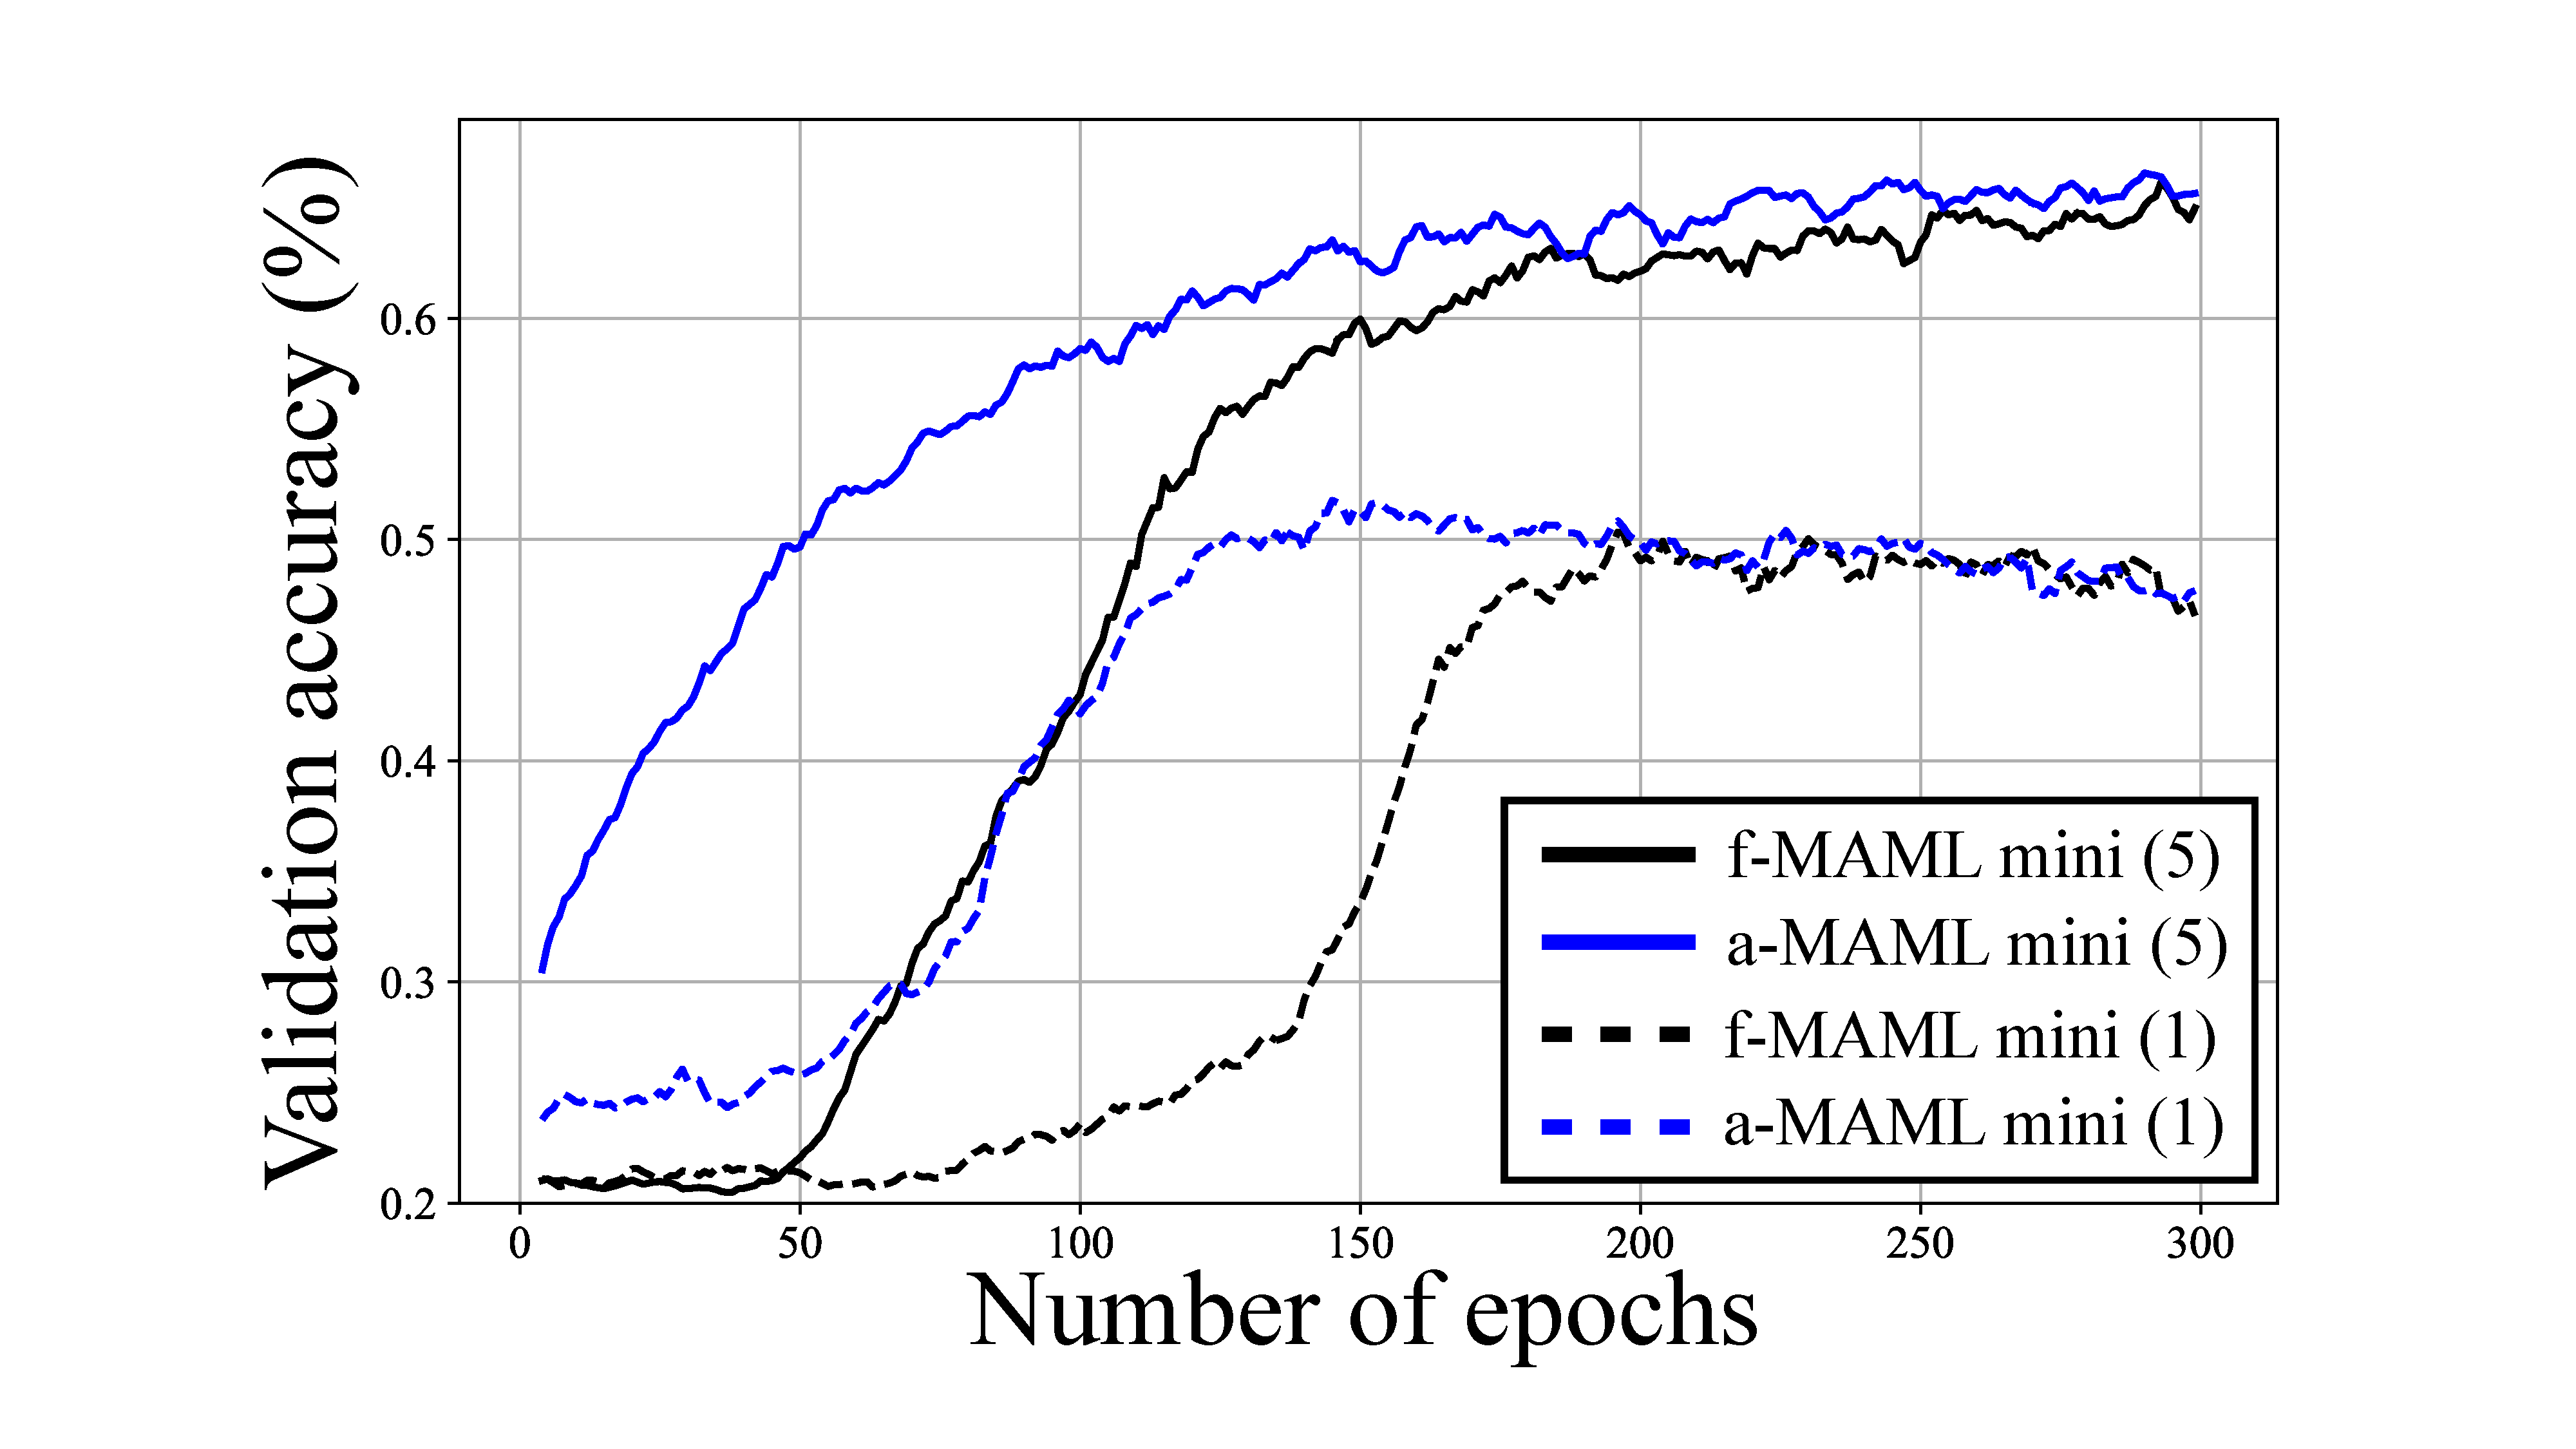
\includegraphics[width=0.45\textwidth]{figure/cropped_convergence.pdf}
\caption{A graph comparing validation accuracy upon training epochs. The numbers in parentheses indicate the number of shots. The validation accuracy is measured in the 5-way case. mini refers MiniImageNet.}
% \vspace{-3mm}
\label{fig:convergence_speed}
\end{figure} 



\subsection{Any-Way, Through the Lens of Ensemble}
\paragraph{Ensemble on Assigned sets.} Our ensemble-based perspective provides insights into the improved performance of our algorithm. As highlighted in Sec.~III.2, 
the flexibility in assigning numeric labels offers a way to generate diverse models without any additional costs.
%we emphasized that varying the assignment of numeric labels can be conceptualized as a mechanism to generate diverse models without additional cost. 
By harnessing the multiple logits derived from the same task set, we can utilize %capitalize on 
these `independent' pieces of information.

Table~\ref{table:ensemble1} corroborates this idea. As the number of assignment sets, \nj{$J$,} increases, %is expanded, 
the performance improves due to the model ensembling with logits generated by each distinct set. With our `any-way' approach, it is possible to generate an `almost' infinite number of such assignment sets, each acting as a representation of an independent model. We conducted various basic ensemble methods and all of those methods have shown promising performance improvements as the number of models increases. Nonetheless, there exists a finite limit due to the inherent \nj{upper bound of ensembling}.
In essence, our methodology harnesses the power of ensemble by utilizing varying numeric label assignments. This diversification, when combined, forms a robust model that is more adaptable and delivers superior performance. Additionally, Table~\ref{table:ablation} supports our analysis, showing a positive correlation between the number of output nodes and performance. This is because an increase in the number of outer nodes leads to more ensembling.
% 앙상블 관점의 접근은 왜 우리의 알고리즘이 이러한 결과를 보여줬는지에 대한 힌트를 제공한다. 
% As stated in Sec.~\ref{sec:anywaymetalearning}, we argued that different assignment of numeric labels can be viewed as creating different models with free. Which means, by leveraging multiple logits on same task set, we can ensemble those 'independent' information. Table~\ref{table:ensemble} hints on this, when we increase the number of assignment set then ensemble with logits which is generated by each assigned set, the performance increased. What's more is that we can generate 'almost' infinite number of assignment set. and each represents independent model. Which means we can (theroritically) incrase the number of independent logits. For example, our any-way trained classifier has the output dimension is 30, and assigned task which has 5 numeric labels. This means, we can initially assign 6 assignment sets. And get corresponding logits, However, we can assign to label different way then optimize again, thereby we can get additional 6 logits.

\begin{table}[]
\centering
% \vspace{-3mm}
\resizebox{\columnwidth}{!}{%
\begin{tabular}{c|cccccc}

train  & \multicolumn{6}{c}{MiniImageNet}                                                                            \\ \hline
test & \multicolumn{3}{c|}{MiniImageNet}                               & \multicolumn{3}{c}{cars}                   \\ \hline
method        & original     & softmax      & \multicolumn{1}{c|}{max}    & original     & softmax      & max    \\ \hline
1             & 65.00    & 65.00     & \multicolumn{1}{c|}{65.00 }    & 47.66  & 47.66  & 47.66  \\
% 1             & 65.00 (0.46)    & 65.00 (0.46)    & \multicolumn{1}{c|}{65.00 (0.46)}    & 47.66 (0.82) & 47.66 (0.82) & 47.66 (0.82) \\
% 2             & 66.20 (0.34)  & 66.18 (0.36) & \multicolumn{1}{c|}{65.11 (0.40)}  & 49.02 (0.66) & 49.01 (0.67) & 47.81 (0.73) \\
2             & 66.20   & 66.18  & \multicolumn{1}{c|}{65.11 }  & 49.02  & 49.01  & 47.81  \\
3             & 66.58   & 66.57  & \multicolumn{1}{c|}{66.22 } & 49.31  & 49.3   & 48.86  \\
% 3             & 66.58 (0.50)  & 66.57 (0.49) & \multicolumn{1}{c|}{66.22 (0.46)} & 49.31 (1.12) & 49.3 (1.09)  & 48.86 (1.11) \\
6             & 66.82 & 66.81  & \multicolumn{1}{c|}{66.54 } & 49.83  & 49.81  & 49.48   \\
12 $\star$           & 66.99  & 66.97  & \multicolumn{1}{c|}{66.69 } & 49.81  & 49.82  & 49.48  \\
18 $\star$           & 66.82  & 66.81  & \multicolumn{1}{c|}{66.59 } & 49.98  & 49.95  & 49.59 
% 6             & 66.82 (0.25) & 66.81 (0.25) & \multicolumn{1}{c|}{66.54 (0.28)} & 49.83 (0.99) & 49.81 (0.97) & 49.48 (0.90)  \\
% 12 $\star$           & 66.99 (0.34) & 66.97 (0.33) & \multicolumn{1}{c|}{66.69 (0.37)} & 49.81 (1.06) & 49.82 (1.07) & 49.48 (1.08) \\
% 18 $\star$           & 66.82 (0.54) & 66.81 (0.55) & \multicolumn{1}{c|}{66.59 (0.61)} & 49.98 (1.04) & 49.95 (1.06) & 49.59 (0.99)
\end{tabular}
}
\caption{Accuracy of a-MAML across various datasets, shots, and ensembling techniques on the 5-way setting. Ensembling methods include: (i) \textit{original}: direct summation of output logits, (ii) \textit{softmax}: \nj{summation of} softmax \nj{outputs} on logits, and (iii) \textit{max}: selection of the maximum output logit per assignment set. The $\star$ refers \nj{to} multiple inner loop\nj{s} for \nj{a} single task for more \nj{ensembling}. The model was trained with 5 shots.}
\label{table:ensemble1}
\end{table}

\paragraph{Ensemble on Different Cardinality Episodes.}
In Fig.~\ref{fig:convergence_speed}, it is evident that our algorithm, a-MAML, converges more rapidly than f-MAML. Beyond its faster convergence, a-MAML also demonstrates superior performance in comparison to f-MAML. This distinction provides insights into the challenges faced during the  training of fixed 10-way 1-shot TieredImageNet \nj{(See the caption of Table \ref{table:GBML_MAIN})}. Specifically, as the complexity of the task increases, the duration of the ``Start-up Stall" phase — where performance remains stagnant after initialization — becomes more pronounced. Given that TieredimageNet is one of the most challenging datasets, primarily due to its expansive semantic class pool (361) and the intricate nature of the task (classifying unseen numeric labels within a single shot), the advantages of a-MAML become even more apparent. By ensembling across different cardinalities, a-MAML swiftly moves past the Start-up Stall phase during simpler tasks like 3-way episodes. This proficiency with easier tasks subsequently empowers the algorithm to tackle harder tasks, such as 9-way episodes, more effectively.

\subsection{Injecting  Semantic information into model}
In our experiments, as detailed in Tables \ref{table:anysemantic} and \ref{table:fixedsemantic}, we found that the integration of semantic class information significantly enhanced the performance of models, especially when tailored for fine-grained datasets. However, the effects of this integration varied depending on the characteristics of the datasets \jh{in any-way case}. %manifested differently based on the nature of the dataset. 
For models trained on coarse-grained datasets \nj{(G$\rightarrow$S)}, there was a potential decrease in generalizability, as evidenced by diminished performance on intricate datasets like ``MiniImageNet". In contrast, models trained on detailed datasets, such as ``Cars" or ``CUB", not only maintained but even demonstrated enhanced versatility across varied test scenarios. This suggests that the subtle intricacies %nuanced specifics 
of fine-grained datasets are further emphasized %accentuated 
with semantic nuances, enabling models to discern delicate %differentiate subtle 
class differences with greater precision.

\paragraph{Mixup: Crafting Geometry into feature embeddings.} 
\yr{While it is generally beneficial} to inject semantic class {information}, there are \yr{some instances where performance degradation is observed.} %of degradation. 
\yr{This occurs due to the inherent nature of features, which do not readily adapt to geometry. Instead, they lie in a smaller manifold, resulting in intricate challenges when capturing their metrics. To mitigate these cases, we could implement techniques commonly used in supervised learning, specifically Mixup, as shown in Table~\ref{table:anysemantic}.}
%We could remedy these cases by implementing techniques commonly used in supervised learning, specifically Mixup, as shown in Table~\ref{table:anysemantic}. %\jh{By doing mixup, we could adapt geometry into feature space.}
% yr: 이 문단을 위로 빼기
%Normally, features do not readily adapt to geometry; they lie in a smaller manifold, and their metrics are intricate to capture. This requires specific methodologies to address \nj{these} challenges, often leading to difficulties in generalization. By introducing Mixup, we can effectively address these challenges.

\yr{Previous} research~\cite{scarcitylabel} has already \yr{employed Mixup} for meta-learning \yr{objectives}. However, \yr{such implementations primarily address data scarcity by increasing the number of shots within a single episode through Mixup.}
%such applications solves the problem by formulating data scarcity, which means, levearaging more shots in single episode by mixup. 
In contrast, our approach \yr{focuses on the} %seeks
the geometry of the feature space without leveraging \yr{additional} %any extra 
shots in individual tasks. As we did not leverage the benefits of additional shots by Mixup, we can apply other mixup methods designed to address dataset scarcity simultaneously; that is, we can anticipate further performance enhancement. 
%\jh{As we \nj{did not} exploit the benefits of additional shots generated through Mixup, We can harness the advantage of other mixup methods which intended to solve dataset scarcity in parallel.}
\begin{table}[t]
\centering
\adjustbox{width=0.40\textwidth}{
\begin{tabular}{c|cc|cc|cc} 
% \toprule
{Way} & \multicolumn{2}{c|}{3} & \multicolumn{2}{c|}{5} & \multicolumn{2}{c}{10} \\
\hline

% \cmidrule(lr){2-3} \cmidrule(lr){4-5} \cmidrule(lr){6-7}
{O \textbackslash  Data} & {mini}  & {cars}  & {mini}  & {cars}  & {mini}  & {cars}  \\ \hline
% \midrule
10       & 76.79         & 60.53 & 63.91         & 46.04 & 46.34         & 30.62  \\
20       & 78.83         & 62.01 & 66.71         & 47.92 & 49.96         & 32.71  \\
30       & 79.06         & 63.58 & 66.73         & 49.80  & 50.28         & 34.82  \\
% \bottomrule
\end{tabular}
}
\caption{Experiments on the number of output nodes $O$. A model was trained on the Mini-ImageNet dataset using an any-way training method, excluding the semantic classifier.}
\label{table:ablation}
\end{table}

Our auxiliary classifier $g_s$ classifies mix-up labels at the same ratio\yr{, thereby reflecting the model's} disentangled feature space \yr{corresponding to} mix ratios in the input spaces. \yr{This enables} the model to adopt a geometric invariance. By increasing such invariance, the model enhances its \nj{generalizability} \yr{while} maintaining its structure.

Table~\ref{table:anysemantic} demonstrates the overall performance improvement achieved with Mixup. However, in some cases \nj{especially} in `Same' scenarios, performance degradation occurs due to the %. This is because there exists a 
trade-off between generality and specificity \cite{theory:specificdataset}. This arises from the fact that, while Mixup enables the adoption of general features, it also leads to the loss of specific features that could be advantageous when applied within the same domain. %당연히좋죠...₩
% Although we could adopt general features through mixup, we lost some specific features that might be helpful when tested within the same domain.

%Table~\ref{table:anysemantic} supports our \nj{hypothesis} \yr{어떤 hypothesis인지 명시해주면 좋을듯}, demonstrating that when the scenario requires generalization to %generalibility do 
%different distributions, performance improves. \yr{여기도 연결성 부족} However, there are cases where performance degrades in the `Same' scenario. \yr{여기도 앞뒤 연결하면 좋을 것 같음} %increases whereby there are cases of performance degradation on same domain scenario. 

% \yr: 이 문단을 두번째 문단으로 올리는 것도 좋을 것 같긴 하다..

%Our approach to Mixup differentiates itself %stands distinct 
%within the Gradient-Based Meta-Learning (GBML) landscape. While many resort to Mixup to mitigate data scarcity and expand %, expanding 
%shot counts in episodes, we chose a different path. \yr{어떻게 다른 path?} We kept the shot count consistent during Mixup, emphasizing the transformation of the feature space over increasing data quantity. This focus, combined with our model's proficiency in extracting semantic information, distinguishes our methodology. % sets our methodology apart.

%\jh{Our auxiliary classifier classifies mix-up labels at the same ratio, ensuring that the combined features from \yr{the} mixed semantic classes accurately \yr{represent} the blending of the actual images. This process allows the feature space \yr{of the model} to adopt a geometric structure. In other words, a model can mirror the intanglement of mix ratios in input spaces. Our approach to Mixup stands distinct in the Gradient-Based Meta-Learning (GBML) landscape. While many resort to Mixup to mitigate data scarcity, expanding shot counts in episodes, we chose a different path. We kept the shot count consistent during Mixup, emphasizing the transformation of the feature space over increasing data quantities. This focus, coupled with our model's adeptness at semantic information extraction, sets our methodology apart. Normally, features do not adapt to geometry; they lie in a smaller manifold, and their metrics are challenging to capture, requiring specific methodologies to address this. This naturally leads to challenges in generalization. By introducing Mixup, we can address these challenges.}
% \jh{Our approach to Mixup stands distinct in the Gradient-Based Meta-Learning (GBML) landscape. While many resort to Mixup to mitigate data scarcity, expanding shot counts in episodes, we chose a different path. We kept the shot count consistent during Mixup, emphasizing the transformation of the feature space over increasing data quantities. This focus, coupled with our model's adeptness at semantic information extraction, sets our methodology apart.}

% Building on the foundation of semantic class insights, we \yr{delved} into \yr{the utilization of} %leveraging 
% the mixup technique, a staple in supervised learning, to enhance our model's generalizability. Our auxiliary classifier's unique architecture, designed to interpret semantic class information, positioned us advantageously to tap into mixup's potential.
% \yr{이 파트도 잘 이해 안 감 한 번 다시 정리해봤으면 좋겠음. 중복되는 내용이 좀 많은 것 같음..}

% \jh{As showcased in Table \ref{table:anysemantic}, the integration of mixup not only amplified performance across the board but also excelled in challenges like 10-way classification, even when confronted with previously uncharted training distributions.}




\section{Conclusion and Future Work}
In this work, we primarily proposed a generalization problem in meta-learning across various task cardinalities. To remedy this issue, we  bring the innate characteristic of episode-based learning, label equivalence. By harnessing label equivalence, we could implement a model capable of dealing with any task cardinality. Our any-way meta-learning surpasses fixed-meta learning, which goes against conventional wisdom. Additionally, we claimed that this equivalence naturally lacks semantic information to classes, thereby we devised a method to inject semantic information into the model. Moreover, our proposed model exhibits some characteristics of supervised learning, prompting us to explore the potential of integrating supervised learning techniques. %Also, as our proposed model partially becomes supervised learning, we showcased the possibility of adopting supervised learning`s technique. 
We envision our paper as a catalyst for raising essential inquiries: `What truly defines meta-learning ability?' and `What unfolds when models are trained with episode-sampled data?'
%We hope our paper can question `What is true meta-learning ability?` and the intention about `What happens if we train model with of episode-sampled-data?`.

Our algorithm is intuitive and straightforward, utilizing a fundamental and general architecture for broad applicability. %we used most basic and general archtecture for wide application.
Additionally, we employed the simplest %used most simple 
ensemble technique, as seen in Table~\ref{table:ensemble1}. As part of our ongoing efforts, we are actively developing more advanced algorithms to harness the potential of this label equivalence and to further enhance the ensemble technique enabled by this equivalence.
\begin{table}[t]
\centering
% \vspace{-3mm}
\resizebox{0.95\columnwidth}{!}{%
\begin{tabular}{l|l|l|l|l}
\multicolumn{1}{c|}{Scenario}   & \multicolumn{1}{c|}{Same}              & \multicolumn{1}{c|}{Same}              & \multicolumn{1}{c|}{G $\rightarrow$ S} & \multicolumn{1}{c}{S $\rightarrow$ G}   \\ \hline
\multicolumn{1}{c|}{Train$\rightarrow$Test} & \multicolumn{1}{c|}{M $\rightarrow$ M} & \multicolumn{1}{c|}{C $\rightarrow$ C} & \multicolumn{1}{c|}{M $\rightarrow$ C} & \multicolumn{1}{c}{C $\rightarrow$ M} \\ \hline
\multicolumn{1}{c|}{f-MAML (1)} & 46.86 (0.95)      & 49.19 (0.56)      & 35.09 (0.66)      & 28.76 (0.91)      \\
\multicolumn{1}{l|}{+semantic}  & 48.32 (0.89)      & 51.21 (0.36)       & 34.65 (0.20)      & 29.48 (0.36)      \\ \hline
\multicolumn{1}{c|}{f-MAML (5)} & 65.41 (1.04)      & 70.42 (0.88)      & 48.07 (1.83)      & 39.41 (0.62)      \\
\multicolumn{1}{l|}{+semantic}  & 66.89 (0.35)      & 71.45 (1.10)      & 46.19 (2.76)      & 40.46 (0.61)     
\end{tabular}
}
\caption{Testing the effectiveness of injecting semantic information to fixed-way meta-learning. The \nj{numbers in parentheses are the number of shots}. M and C refer \nj{to} MiniImageNet and Cars, \nj{respectively. `+semantic' indicates a model trained with an additional semantic classifier with the $L_{semantic}$ loss. } Note that the class in the test phase is totally unseen during training.} % in the Train Test section.}
\label{table:fixedsemantic}
\end{table}

\section{Acknowledgements}
This work was supported by IITP grants (2022-0-00953, 2021-0-01343) and NRF grant (2021R1A2C3006659), all funded by MSIT of the Korean Government.

\clearpage
%We remain devising more sophisticated algorithm to exploit this label equivalence, and ensemble technique which is achived by this equivalence as future research.

% My first thought is that previous GBML consists of sampling task with same number of classes and 
% same number of samples. This means the label itself does not contain any information. 
% So my research tries to convey the information of label without changing the algorithm itself.

% So I made auxiliary classifier, which classifiers true_label itself. Which means, a class is 
% assigned to specific label. Where a class is assiged randomly to each task in GBML.
% A auxiliary classifier is trained to classify the true_label. To do so, Additional loss is added
% to the original loss. In the inner loop, auxiliary classifier is trained to classify the true_label.
% In order to prevent this loss harms the original loss, only auxiliary classifier is trained with this loss.
% Also, as this classifier is similar to normal supervised learning setting, we can use some techniques
% of supervised learning. In this paper, we use the technique of mixup.

% The second part is that previous GBML is not suitable for the task with different number of classes.
% For example, when we train the model with 5-way 5-shot, we can only use the task with 5 classes.
% We cannot use the task with 6 classes. So I made a model that can train with different number of classes.
% Which means, a real meta-model should classify any number of classes. We present the technique of it 
% without changing sampling task method itself. Which means, it can classify any ways with fixed-way training.
% To do so, we adopt a classifier which outputs more then the number of classes. for example,, suppose
% the classifier outputs 30 classes. At every task, we randomly select 5 classes from 30 classes. 
% Then, we train the model with 5-way 5-shot. In this way, we can train the model with different number of classes.
% As the index itself has no meaning, we can use this technique. Also, in order to prevent the model losses

% \section{Future work}

% 1. Doing ensemble is really straightforward in our section, more methods can be studied for future work.
% 2. Also, we just showcased the possibility of integration between supervison and meta learning.

% Someone can think this feature prevents overfitting and helps generalization. However, any model cannot learn
% The outer space of convex hall. The more we provide the data, the more the model can learn.

% Sum up, the task sampling method in GBML has double-edged feature. It makes GBML possible, but it lacks the information.
% In this paper, we propose two techniques which exploits the double-edged feature of task sampling method in GBML.
% First, we propse a model which can classify any number of classes without changing the task sampling method itself.
% which means we can classify any number of classes with fixed-way training. As we remained the task sampling method, this technique can be applied to any GBML model. This technique was possible as the label itself does not contain any information. Second, we propolse an algorithm which injects the information of label to the model by adding lightweight classifier. This method requare little computational burden. Also, as this classifier is similar to normal supervised learning setting,
% We can apply the technique of supervised learning. In this paper, we use the technique of mixup, which is known to be effective
% and common technique in supervised learning. We can apply this technique if we have labeled data, also, we can expect
% additional performance gain by adopting techniques in supervised learning which is not introduced in this paper.

% You can achieve all of the above by enabling the \texttt{submission} option when loading the \texttt{aaai24} package:

% \begin{quote}\begin{scriptsize}\begin{verbatim}
% \documentclass[letterpaper]{article}
% \usepackage[submission]{aaai24}
% \end{verbatim}\end{scriptsize}\end{quote}

% The remainder of this document are the original camera-
% ready instructions. Any contradiction of the above points
% ought to be ignored while preparing anonymous submis-
% sions.
% \begin{table*}[]
% \caption{\jh{Accuracy of \nj{a-}MAML across various datasets, shots, and ensembling techniques \nj{on the 5-way setting.} Ensembling methods include: (i) \textit{Original} - direct summation of output logits, (ii) \textit{Softmax} - prior \nj{(??)} softmax operation on logits, and (iii) \textit{Max} - selection of the maximum output logit per assignment set.}}
% \centering
% \begin{center}
%     \adjustbox{max width=1.0\textwidth}{
% \begin{tabular}{c|llllll|llllll}
% shot &
%   \multicolumn{6}{c|}{1 shot} &
%   \multicolumn{6}{c}{5 shot} \\ \hline
% train dataset &
%   \multicolumn{6}{c|}{MiniImageNet} &
%   \multicolumn{6}{c}{Cars} \\ \hline
% test dataset &
%   \multicolumn{3}{c|}{MiniImageNet} &
%   \multicolumn{3}{c|}{Cars} &
%   \multicolumn{3}{c|}{MiniImageNet} &
%   \multicolumn{3}{c}{Cars} \\ \hline
% method &
%   \multicolumn{1}{c}{original} &
%   \multicolumn{1}{c}{softmax} &
%   \multicolumn{1}{c|}{max} &
%   \multicolumn{1}{c}{original} &
%   \multicolumn{1}{c}{softmax} &
%   \multicolumn{1}{c|}{max} &
%   \multicolumn{1}{c}{original} &
%   \multicolumn{1}{c}{softmax} &
%   \multicolumn{1}{c|}{max} &
%   \multicolumn{1}{c}{original} &
%   \multicolumn{1}{c}{softmax} &
%   \multicolumn{1}{c}{max} \\ \hline
% 1 &
%   47.64 (0.53) &
%   47.64 (0.53) &
%   \multicolumn{1}{l|}{47.64 (0.53)} &
%   34.45 (0.21) &
%   34.45 (0.21) &
%   34.45 (0.21) &
%   38.66 (1.05) &
%   38.66 (1.05) &
%   \multicolumn{1}{l|}{38.66 (1.05)} &
%   67.18 (1.21) &
%   67.18 (1.21) &
%   67.18 (1.21) \\
% 2 &
%   48.11 (0.3) &
%   48.11 (0.28) &
%   \multicolumn{1}{l|}{47.56 (0.28)} &
%   35.05 (0.12) &
%   35.03 (0.12) &
%   34.59 (0.07) &
%   39.9 (0.83) &
%   39.91 (0.85) &
%   \multicolumn{1}{l|}{38.84 (0.96)} &
%   68.65 (0.9) &
%   68.7 (1.06) &
%   66.89 (1.19) \\
% 3 &
%   48.02 (0.8) &
%   48.03 (0.78) &
%   \multicolumn{1}{l|}{47.84 (0.82)} &
%   35.05 (0.2) &
%   35.03 (0.2) &
%   34.84 (0.24) &
%   40.13 (0.83) &
%   40.19 (0.87) &
%   \multicolumn{1}{l|}{39.66 (0.86)} &
%   69.52 (0.8) &
%   69.58 (0.99) &
%   68.99 (1.09) \\
% 6 &
%   48.24 (0.34) &
%   48.23 (0.35) &
%   \multicolumn{1}{l|}{48.13 (0.35)} &
%   35.11 (0.06) &
%   35.1 (0.05) &
%   34.98 (0.08) &
%   40.8 (0.9) &
%   40.8 (0.98) &
%   \multicolumn{1}{l|}{40.44 (1.12)} &
%   70.24 (0.84) &
%   70.32 (1.01) &
%   69.92 (1.09) \\
% 12 &
%   48.41 (0.29) &
%   48.4 (0.3) &
%   \multicolumn{1}{l|}{48.26 (0.38)} &
%   35.18 (0.1) &
%   35.16 (0.12) &
%   35.06 (0.13) &
%   40.9 (0.78) &
%   40.93 (0.85) &
%   \multicolumn{1}{l|}{40.57 (0.96)} &
%   70.12 (1.07) &
%   70.19 (1.2) &
%   69.77 (1.34) \\
% 18 &
%   48.55 (0.34) &
%   48.56 (0.34) &
%   \multicolumn{1}{l|}{48.45 (0.34)} &
%   35.27 (0.17) &
%   35.25 (0.16) &
%   35.16 (0.19) &
%   40.63 (0.6) &
%   40.66 (0.66) &
%   \multicolumn{1}{l|}{40.33 (0.72)} &
%   70.27 (0.88) &
%   70.37 (1.05) &
%   69.95 (1.22)
% \end{tabular}
% }
% \end{center}
% \caption{\hh{  This table indicates the accuracy of ensembled models for different dataset, shots, and ensembling methods. The data above were experimented with three different seeds, and the numbers within parentheses represent the standard deviations, measured in percentage units. \\
% As explained above, increasing the number of assignment sets is equivalent to increasing the model output logits, which is same as ensembling across independent models. We test the consequence of ensemble method on the any-way MAML model trained on MiniImageNet and Cars dataset. To ascertain the model's robustness, we evaluate it across varying shot numbers, datasets, and ensembling techniques. We ensemble the models on three different methods: the straightforward summation of output logits for each corresponding assignment set (referred to as 'original'), the application of a softmax operation before aggregating the logits ('softmax'), and selecting the maximum output logit for each assignment set and subsequently according it equal voting power for the output class ('max'). The numerical values on the vertical axis indicate the number of assignment sets generated, representing the number of ensembles. From the result of this table we can observe that the accuracy rises with a increase in the amount of ensemble, while remaining independent of other conditions. This stands as one of the most significant advantages of anyway-MAML , as it enables performance enhancement through straightforward ensemble methods of multiple assignment sets without incurring substantial computation costs.\\
% The methods of ensembling could be thought of filters which are operated before the ensemble process. For example the softmax operation is a filter which applies greater weight to larger values, and the max operation is a filter which takes only the maximum value and makes it a unit constant. As we move from original, softmax, max method, the outliers of each outputs tend to diminish. The observation that an increase in the number of ensembles leads to a higher accuracy, and this trend remains consistent across different methods, suggests that the model is highly robust to outliers.}}
%\label{table:GBML_CROSS}
%\label{table:ensemble}
%\end{table*}


\bibliography{reference/aaai24}

\newpage
\appendix
\section{good}

\end{document}
